
\documentclass{article}
\usepackage{anyfontsize}
\usepackage[UTF8]{ctex} % 如果需要支持中文
\usepackage{fontspec} 
\usepackage{bookmark}
% \setCJKmainfont{SourceHanSansCN-Light}[
%     BoldFont=SourceHanSansCN-Medium
% ]

\usepackage[a4paper, left=0.1in, right=0.1in, top=0.05in, bottom=0.05in]{geometry} % 设置四边页边距为0.1英寸{geometry} % 设置页边距为0.5英寸
\usepackage{enumitem} % 用于自定义列表
\usepackage{amsmath}  % 数学公式支持

\setlength{\parindent}{0pt} % 不缩进
\usepackage{etoolbox} % 用于列表操作
%调整类代码
\usepackage{comment}
\usepackage{tocloft} % 用于定制目录样式
\usepackage{hyperref} %不需要目录盒子注释这
\usepackage{ifthen}
\usepackage{tikz}
\usepackage{titletoc}
\usepackage{graphicx}
\usepackage{float}
\usepackage{amssymb}  % 提供数学符号，包括\therefore
\usepackage{xcolor}  % 提供颜色支持，用于\textcolor命令
%目录设定
%快捷键 CMD + / 注释
%  \renewcommand{\cftdot}{} % 隐藏目录中的页码
%  \cftpagenumbersoff{section}
%  \cftpagenumbersoff{subsection}
%  \makeatletter
%  \renewcommand{\@pnumwidth}{0em}  % 设置页码宽度为0
%  \renewcommand{\@tocrmarg}{0em}   % 设置右边距为0
%  \makeatother
 
\graphicspath{{images/}}

\usepackage{environ}

\newif\ifshowcontent  % 定义一个条件判断变量
\showcontenttrue    % 设置为 false，隐藏所有 question 环境的内容

\newcounter{question} % 题目计数器
\setcounter{question}{0}
\NewEnviron{question}{%
    \ifshowcontent
    \vspace{1cm}\stepcounter{question}\textbf{\thequestion.} \BODY\par % 如果显示内容，则输出
    \fi
}

\NewEnviron{choices}{%
    \ifshowcontent
        \begin{enumerate}[label=\Alph*., leftmargin=*]
            \BODY
        \end{enumerate}\par
    \fi
}

\NewEnviron{correctanswer}{%
    \ifshowcontent
        \textbf{答案:}\BODY\par
    \fi
}



\newenvironment{explanation}
{\textbf{解析:}\par}
{\par}



% % 新增考察方面命令
% \newcommand{\checklist}[1]{
%     \textbf{考察:} #1 \par % 在题目下方显示考察方面
%     \addcontentsline{toc}{subsection}{题号\thequestion 考察: #1} % 将考察内容添加到目录
%     \vspace{2em} % 添加1em的垂直空间
% }

% \graphicspath{{images/}} %统一







\newcommand{\tocstar}[1]{%
    \texorpdfstring{%
        \protect\textcolor{blue}{%
            \ifnum#1=1 {\protect\textbf{$[\blacksquare\square\square\square\square]$}}\fi%
            \ifnum#1=2 {\protect\textbf{$[\blacksquare\square\square]$}}\fi%
            \ifnum#1=3 {\protect\textbf{$[\blacksquare\blacksquare\square]$}}\fi%
            \ifnum#1=4 {\protect\textbf{$[\blacksquare\blacksquare\blacksquare]$}}\fi%
            \ifnum#1=5 {\protect\textbf{$[\blacksquare\blacksquare\blacksquare\blacksquare\blacksquare]$}}\fi%
        }%
    }{*}%
}



% 在导言区添加以下代码（放在 \begin{document} 之前）
\makeatletter
% 定义新的目录格式
\newcommand{\listbookname}[1]{Book#1 目录}

% 设置目录格式
\renewcommand{\cftsecleader}{\cftdotfill{\cftdotsep}} % 添加虚线
\renewcommand{\cftsecpagefont}{\normalfont}  % 页码字体
\setlength{\cftsecindent}{1em}     % 缩进
\setlength{\cftsecnumwidth}{2.3em}   % 编号宽度
\setlength{\cftbeforesecskip}{1pt}   % 减小节之间的垂直间距

% 为每个book定义新的目录格式
\@for\i:={1,2,3,4}\do{
    \expandafter\newcommand\csname book\i toc\endcsname{\section*{\mdseries\normalfont\listbookname{\i}}}
    \expandafter\newcommand\csname l@book\i\endcsname{\@dottedtocline{1}{1em}{2em}}
}

% 定义四个目录命令
\newcommand{\bookonecontents}{%
    \section*{Foundations of Risk Management 目录}
    \@starttoc{book1}%
}

\newcommand{\booktwocontents}{%
    \section*{Quantitative Analysis 目录}
    \@starttoc{book2}%
}

\newcommand{\bookthreecontents}{%
    \section*{Financial Markets and Products 目录}
    \@starttoc{book3}%
}

\newcommand{\bookfourcontents}{%
    \section*{Valuation and Risk Models 目录}
    \@starttoc{book4}%
}
\makeatother
% 修改 checklist 命令
\newcommand{\checklist}[3]{%
    \textbf{考察:} #1 
    \hspace{1em}
    \textbf{重要程度：}\textcolor{blue}{%
        \ifthenelse{\equal{#2}{1}}{$[\blacksquare\square\square\square\square]$}{%
        \ifthenelse{\equal{#2}{2}}{$[\blacksquare\square\square]$}{%
        \ifthenelse{\equal{#2}{3}}{$[\blacksquare\blacksquare\square]$}{%
        \ifthenelse{\equal{#2}{4}}{$[\blacksquare\blacksquare\blacksquare]$}{%
        \ifthenelse{\equal{#2}{5}}{$[\blacksquare\blacksquare\blacksquare\blacksquare\blacksquare]$}{}}}}}%
    }\par
    \textbf{科目:} \ifthenelse{\equal{#3}{1}}{Foundations of Risk Management}{\ifthenelse{\equal{#3}{2}}{Quantitative Analysis}{\ifthenelse{\equal{#3}{3}}{Financial Markets and Products}{Valuation and Risk Models}}}\par
    % 根据不同的 BOOK 添加到相应的目录
    \ifthenelse{\equal{#3}{1}}{\addcontentsline{book1}{subsection}{题号\thequestion 考察: #1 \tocstar{#2}}}{}
    \ifthenelse{\equal{#3}{2}}{\addcontentsline{book2}{subsection}{题号\thequestion 考察: #1 \tocstar{#2}}}{}
    \ifthenelse{\equal{#3}{3}}{\addcontentsline{book3}{subsection}{题号\thequestion 考察: #1 \tocstar{#2}}}{}
    \ifthenelse{\equal{#3}{4}}{\addcontentsline{book4}{subsection}{题号\thequestion 考察: #1 \tocstar{#2}}}{}
}
% \let\oldtextbf\textbf
% % 重定义 \textbf 命令，使其带有颜色
% \renewcommand{\textbf}[1]{\textcolor{deepblue}{\oldtextbf{#1}}}











\begin{document}
%  %\fontsize{23}{31}\selectfont
%  \tableofcontents % 添加目录
% \newpage
% %\pagestyle{empty}

  % 在需要显示目录的位置添加
  \bookonecontents
  \newpage
  \booktwocontents
  \newpage
  \bookthreecontents
  \newpage
  \bookfourcontents
  
      \newpage
  
  
  \newpage
  
  

  

  % --- Question 1 ---
  \begin{question}
      Consider an exposure with a value of $\$30.0$ million. In L(+)/P(-) format, its expected loss is $4.0\%$ with volatility of $15.0\%$; i.e., $\mu(L/P) = +4.0\%$, $\sigma = 15.0\%$. Conveniently, the exposure happens to have a normal distribution. Which is \textbf{nearest} to the single-period $97.5\%$ expected shortfall (ES)?
  \end{question}
  
  \begin{choices}
      \item 6.60 million
      \item 9.38 million
      \item 11.72 million
      \item 14.50 million
  \end{choices}
  
  \begin{correctanswer}
  C
  \end{correctanswer}
  
  \begin{explanation}
      \textbf{C选项正确。} If the distribution is normal, the $97.5\%$ ES is approximated by the $99.0\%$ VaR.
      In this case, we can use $\$30.0 * (4.0\% + 15\% * 2.33) = \$30.0 * 38.950\% = \$11.69$.
      The exact $97.5\%$ ES is given by $\$11.7210$, so that is given as the correct choice.
  \end{explanation}
  
  \checklist{Market Risk}{3}{2}
  
  % --- Question 2 ---
  \begin{question}
      Among its financial positions, Zapex Financial Corporation has written a call, entered into an interest rate swap, and written a credit default swap. Among these (the following) four positions, which is the BEST example of wrong-way risk?
  \end{question}
  
  \begin{choices}
      \item Zapex has written (aka, sold) a call option to a counterparty in the same industry
      \item Zapex is the fixed-rate payer in an interest rate swap during an economic recovery
      \item Zapex has written (aka, sold) a credit default swap (CDS) to counterparty whose credit quality is positively correlated with the reference entity
      \item Zapex has a position in a forward currency contract where its mark-to-market gain is positively correlated with the counterparty's default probability
  \end{choices}
  
  \begin{correctanswer}
      D
  \end{correctanswer}
  
  \begin{explanation}
      \textbf{D选项正确。} Zapex has a position in a forward currency contract where its mark-to-market gain is positively correlated with the counterparty's default probability.
      
      Wrong-way (credit) risk is adverse correlation between the exposure and the credit quality, so wrong-way risk is a positive (negative) correlation between exposure and default probability (credit quality). This is wrong-way risk because greater exposure is associated with a lower likelihood of payment. Algebraically, wrong-way (or right-way) risk is some dependence between exposure/EAD and PD. We normally write $EL\% = PD \times EAD$ but that assumes independence between PD and EAD, so a way to think about WWR is simply when $EL > PD \times EAD$, because $EL \neq PD \times EAD$ is also a condition for non-independence.
      
      In regard to (A), (B) and (C), each is an example of RIGHT-WAY risk.
  \end{explanation}
  
  \checklist{Credit Risk}{3}{3}
  
  % --- Question 3 ---
  \begin{question}
  In December 2017, the Basel Committee (BCBS) made several revisions to the Basel III framework. This included revisions to both the standardized approach to credit risk (``Credit risk accounts for the bulk of most banks' risk-taking activities and hence their regulatory capital requirements. The standardized approach is used by the majority of banks around the world, including in non-Basel Committee jurisdictions,'' wrote the Committee) and the internal ratings-based (IRB) approaches to credit risk (``The financial crisis highlighted a number of shortcomings related to the use of internally modeled approaches for regulatory capital, including the IRB approaches to credit risk. These shortcomings include the excessive complexity of the IRB approaches, the lack of comparability in banks' internally modeled IRB capital requirements and the lack of robustness in modelling certain asset classes,'' wrote the Committee).$^1$
  
  In regard to these December 2017 revisions to credit risk approaches in Basel III, which of the following statements is TRUE?
  
  $^1$ ``High-level summary of Basel III reforms,'' (Basel Committee on Banking Supervision Publication, December 2017)
  \end{question}
  
  \begin{choices}
      \item In the standardized approach (SA) for residential real estate exposures, the risk weights are lower if the loan-to-value (LTV) falls into a lower band
      \item The standardized approach (SA) eliminated the treatment of unrated exposures because all exposures are required to have an external credit rating
      \item The internal ratings-based (IRB) approach removed the option to use the foundation IRB (F-IRB) because the advanced IRB (A-IRB) must be used for all asset classes
      \item The internal ratings-based (IRB) approach removed the parameter input floors (in the case of PD, LGD, and EAD) to increase RWA variability across different banks
  \end{choices}
  
  \begin{correctanswer}
  A
  \end{correctanswer}
  
  \begin{explanation}
  \textbf{Option A is correct.} In the standardized approach (SA) for residential real estate exposures, the risk weights is lower if the loan-to-value (LTV) falls into a lower band.
  
  See below. Writes BCBS (High-level summary of Basel III reforms, December 2017): ``For residential real estate exposures, more risk-sensitive approaches have been developed, whereby risk weights vary based on the LTV ratio of the mortgage (instead of the existing single risk weight) and in ways that better reflect differences in market structures.''
  
  \begin{figure}[H]
      \centering
      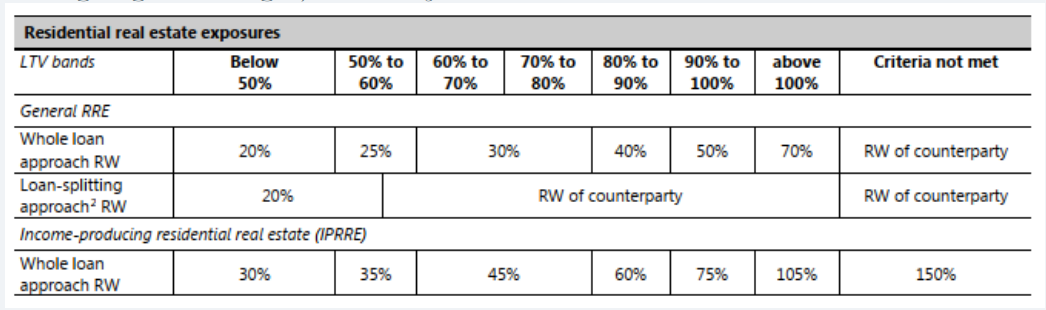
\includegraphics[width=0.6\textwidth]{2·3.png}
  \end{figure}
  
  In regard to (B), (C) and (D), each is FALSE. Instead, the following are true:
  \begin{itemize}
      \item The Basel III reforms included a more granular approach to unrated exposures and reduced the ``mechanistic reliance on credit ratings''
      \item In regard to the internal ratings-based approaches, GARP writes, ``the financial crisis highlighted a number of shortcomings related to the use of internally modeled approaches for regulatory capital, including the IRB approaches to credit risk. These shortcomings include the excessive complexity of the IRB approaches, the lack of comparability in banks' internally modeled IRB capital requirements and the lack of robustness in modelling certain asset classes. To address these shortcomings, the Committee has made the following revisions to the IRB approaches: (i) removed the option to use the advanced IRB (A-IRB) approach for certain asset classes; (ii) adopted ``input'' floors (for metrics such as probabilities of default (PD) and loss-given-default (LGD)) to ensure a minimum level of conservatism in model parameters for asset classes where the IRB approaches remain available; and (iii) provided greater specification of parameter estimation practices to reduce RWA variability.'' --- Source: 2020 FRM Part II: Operational Risk and Resiliency, 10th Edition.
      \item In regard to the Specification of Input Floors: ``The revised IRB framework also introduces minimum floor values for bank-estimated IRB parameters that are used as inputs to the calculation of RWA. These include PD floors for both the F-IRB and A-IRB approaches, and LGD and EAD floors for the A-IRB approach. In some cases, these floors consist of recalibrated values of the existing Basel II floors. In other cases, the floors represent new constraints for banks' IRB models.'' --- Source: 2020 FRM Part II: Operational Risk and Resiliency, 10th Edition.
  \end{itemize}
  \end{explanation}
  
  \checklist{Operational Risk and Resiliency}{3}{2}
  
  % --- Question 4 ---
  \begin{question}
      An asset that is not very liquid is quoted bid $\$89.00$, offer $\$96.00$. Which is \textbf{nearest} to the proportional bid-offer spread?
  \end{question}
  
  \begin{choices}
      \item 0.0378
      \item 0.0757
      \item 0.1538
      \item 7.000
  \end{choices}
  
  \begin{correctanswer}
      B
  \end{correctanswer}
  
  \begin{explanation}
      \textbf{B选项正确。} 0.0757. Because $(96.00 - 89.00)/92.50 = 0.075676$
      
      According to Hull (24.1.2. Measuring Market Liquidity), the two measures of bid-offer spread are:
      \begin{itemize}
          \item Dollar bid-offer spread $= p =$ Offer price -- Bid price
          \item Proportional bid-offer spread $= s =$ (Offer price -- Bid price) / Mid-market price
      \end{itemize}
      
      (Source: John C. Hull, Risk Management and Financial Institutions, 5th Edition (Hoboken, NJ: John Wiley \& Sons, 2018))
  \end{explanation}
  
  \checklist{Market Liquidity}{3}{2}
  
  % --- Question 5 ---
  \begin{question}
      Richard conducted a factor regression for his firm's Flagship Portfolio. He used the three-factor Fama-French specification where the factors are MKT (the market), SMB (small stocks minus big stocks), and HML (value stocks minus growth stocks). His factor regression results are displayed below.
      \begin{figure}[H]
          \centering
          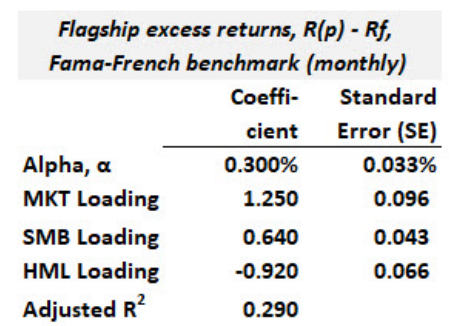
\includegraphics[width=0.6\textwidth]{2·5.png} 
      \end{figure}
      Please note the regression is based on monthly returns. Each of the following statements is TRUE about these factor regression results EXCEPT which is false?
  \end{question}
      
      \begin{choices}
          \item The portfolio's style appears to growth-oriented, small-cap
          \item This portfolio manager(s) appear to be skillful; that is, the alpha is significant
          \item The low adjusted $R^2$ and low standard errors imply these factors are not appropriate to this portfolio
          \item The implied CAPM benchmark is leveraged as it borrows cash (i.e., T-bills) to invest more than 100\% (i.e., $> \$1.0$) in the market portfolio
      \end{choices}
      
      \begin{correctanswer}
      C
      \end{correctanswer}
      
      \begin{explanation}
      \textbf{C选项正确。} C. FALSE: The factors are each significant and the adjusted $R^2$ is relatively high for empirical finance. In regard to (A), (B) and (D), each is true.
      \end{explanation}
      
  \checklist{Finance: Portfolio Management}{3}{2}
  
  % --- Question 6 ---
  \begin{question}
      The riskfree rate is $5.0\%$ while the current stock price is $\$80.00$. Two most liquid options both have a strike price of $\$70.00$ such that the ratio $K/S(0) = 0.90$. In addition to the same strike price, both options have the same maturity of three months, $T = 0.25$ years. The implied volatility of the call is $30.0\%$, and the implied volatility of the put is $38.0\%$. What is the trade that exploits this scenario, if any?
  \end{question}
  
  \begin{choices}
      \item Buy call, sell put, and short the stock
      \item Buy put, sell call, and buy the stock
      \item Buy the call, buy the put, and short a straddle
      \item Sell the call, sell the put, and buy a straddle
  \end{choices}
  
  \begin{correctanswer}
      A
  \end{correctanswer}
  
  \begin{explanation}
      \textbf{A选项正确。} True: Buy call, sell put, and short the stock
  \end{explanation}
  
  \checklist{Derivatives: Options}{3}{2}
  
  % --- Question 7 ---
  \begin{question}
      Consider a netting set with two derivative positions: an interest rate swap (IRS) with a marginal CVA of $-1.450$ and a cross-currency swap (CCS) with a marginal CVA of $-1.550$. If the first transaction is the cross-currency swap (CCS) and its incremental CVA is $-2.100$, then what is the incremental CVA of the IRS?
  \end{question}
  
  \begin{choices}
      \item -0.900
      \item -1.100
      \item -1.550
      \item -2.220
  \end{choices}
  
  \begin{correctanswer}
  A
  \end{correctanswer}
  
  \begin{explanation}
      \textbf{A选项正确。} The total CVA is the sum of marginal CVAs and therefore must be $-1.450 + (-1.550) = -3.000$. The incremental CVAs must sum to the total (netted) CVA such that, if the IRS is second in sequence, its incremental CVA is equal to $-3.000 - (-2.100) = -0.900$.
  \end{explanation}
  
  \checklist{Credit Risk}{1}{1}
  
  % --- Question 8 ---
  \begin{question}
      The central feature of Basel III's first pillar is the regulatory capital (i.e., CET1, Tier 1, and total capital) requirements which require minimum fractions of risk-weighted assets (RWA). In addition to these minimums, as of early 2019 (when the buffers were fully phased in), Basel specifies three buffers: the capital conservation buffer (CCB), the G-SIB buffer, and the countercyclical buffer (CCyB). This is all very confusing, so you ask your colleague Mary to summarize these additional buffers and their motivations. She makes the following five points:
  
      \begin{itemize}
          \item[I.] For all three, the additional buffer must be CET1
          \item[II.] For all three, breach of the buffer requirements implies the bank’s ability to pay dividends will be restricted
          \item[III.] The CCB requires an additional $2.5\%$ of CET1 capital and is meant to ensure that banks have an additional layer of usable capital that can be drawn down when losses are incurred.
          \item[IV.] The additional G-SIB requirement includes five buckets $\{1.0\%, 1.5\%, 2.0\%, 2.5\%, \text{or } 3.5\%\}$ https://www.bis.org/fsi/fsisummaries/g-sib\_framework.htm and is meant to reduce the likelihood and severity of the failure of a global systemically important financial institution
          \item[V.] The CCyB requirement varies between zero and $2.5\%$ and is meant to protect the banking sector from periods of excess aggregate credit growth that have often been associated with the build-up of system-wide risks
      \end{itemize}
  
      Is Mary correct in her summary?
  \end{question}
  
  \begin{choices}
      \item No, unfortunately, none of her statements is correct
      \item I. and II. are correct, but the others (III., IV., and V.) are wrong
      \item III., IV., and V. are correct, but the others (I. and II.) are wrong
      \item Yes, all five statements are correct
  \end{choices}
  
  \begin{correctanswer}
      D
  \end{correctanswer}
  
  \begin{explanation}
      \textbf{D选项正确。} Yes, all five statements are correct
      \begin{itemize}
          \item In regard to true statements (I.) and (II.), the capital conservation buffer (CCB), the G-SIB buffer, and the countercyclical buffer (CCyB) each require common equity Tier 1 (CET1) which is a buffer of the highest quality. Further, breach of any of them implies restrictions on dividend payments (in addition to other supervisor tools such as restriction on executive bonuses)
          \item In regard to true statement (III.), the BCBS says that “the capital conservation buffer [CCB] was introduced to ensure that banks have an additional layer of usable capital that can be drawn down when losses are incurred” (see https://www.bis.org/fsi/fsisummaries/b3\_capital.htm) and GARP says “In the case of the CCB, the rationale roughly follows that for the Prompt Corrective Action (PCA) system built into U.S. capital regulation beginning in 199; i.e., a bank with ratios that begin to approach the minimums should be subject to increasingly stringent supervisory intervention in order to induce a return to well-capitalized status).”– 2020 FRM Part II: Operational Risk and Resiliency, 10th Edition.
          \item In regard to true statement (IV.), the G-SIB requirement includes five buckets $\{1.0\%, 1.5\%, 2.0\%, 2.5\%, \text{or } 3.5\%\}$ and, explains GARP, “In the case of the G-SIB buffer, the rationale is similar to that for the CCB but also recognizes the very large costs to society of distress at G-SIBs (and the higher volatility of losses at some of them). Thus, larger buffers are specified to further reduce the chance of failure.”
          \item In regard to true statement (V.), “The CCyB [countercyclical capital buffer] has two rationales. One is to provide an instrument for macroprudential restraint of overheating; the other is attentive to the cost of capital,” says GARP. Further, explains BCBS, “The countercyclical capital buffer [CCyB] aims to ensure that banking sector capital requirements take account of the macro-financial environment in which banks operate. Its primary objective is to use a buffer of capital to achieve the broader macroprudential goal of protecting the banking sector from periods of excess aggregate credit growth that have often been associated with the build-up of system-wide risk. Due to its countercyclical nature, the countercyclical capital buffer regime may also help to lean against the build-up phase of the credit cycle in the first place. In downturns, the regime should help to reduce the risk that the supply of credit will be constrained by regulatory capital requirements that could undermine the performance of the real economy and result in additional credit losses in the banking system.” See https://www.bis.org/bcbs/ccyb/
      \end{itemize}
      Keep in mind the basic requirements of these three additional buffers: the CCB requires $+2.5\%$ CET1; the G-SIB requires either $\{+1.0\%, +1.5\%, +2.0\%, +2.5\%, \text{or } +3.5\%\}$ depending on the bank’s score (see https://trtl.bz/fsb-g-sibs); and the CCyB requires between zero and $2.5\%$.
  \end{explanation}
  
  \checklist{Finance: Regulatory Capital}{3}{2}
  
  % --- Question 9 ---
  \begin{question}
      A portfolio holds 100,000 shares of a stock and this single position has a value of $\$3.0$ million. The stock is quoted bid $\$29.00$, offer $\$31.00$. The stock's daily volatility is $1.43\%$ or 143 basis points. For purposes of value at risk (VaR), we will assume the stock's arithmetic returns are normally distributed (aka, normal VaR) and the expected daily return rounds to zero (under these assumptions absolute VaR is identical to relative VaR). Which is \textbf{NEAREST} to the position's one-day $99.0\%$ confident liquidity-adjusted value at risk (LVaR)?
  \end{question}
  
  \begin{choices}
      \item $\$15,000$
      \item $\$80,000$
      \item $\$200,000$
      \item $\$1.0$ million
  \end{choices}
  
  \begin{correctanswer}
      C
  \end{correctanswer}
  
  \begin{explanation}
      \textbf{Option C is correct.} The one-day $99.0\%$ VaR is given by $-0 + 1.43\% * 2.326 * \$3.0 \text{ million} = \$99,800$.
      
      The liquidity cost (LC) is given by $(31.00 - 29.00)/30.00 * 0.5 * \$3.0 \text{ million} = \$100,000$.
      
      The one-day $99.0\%$ VaR is therefore $99,800 + 100,000 = 199,800$
  \end{explanation}
  
  \checklist{Market Risk: Liquidity Risk}{3}{2}
  
  % --- Question 10 ---
  \begin{question}
      According to Grinold, typical or illustrative information ratios (IR) include: 0.500 is good, 0.750 is very good and 1.00 is exceptional. In regard to risk aversion, $\lambda$, 0.150 is restrained, 0.100 is moderate, and 0.050 is aggressive. Patricia is a manager with a “very good” information ratio of 0.750 and a “moderate” risk aversion of 0.10. If she shifts from this moderate risk aversion to an aggressive risk aversion of 0.050, what is the impact on the optimal level of active risk?
  \end{question}
  
  \begin{choices}
      \item No effect
      \item Optimal active risk reduces by one-half
      \item Optimal active risk Increases by about +41\%
      \item Optimal active risk doubles
  \end{choices}
  
  \begin{correctanswer}
  D
  \end{correctanswer}
  
  \begin{explanation}
      \textbf{D选项正确。} True: Optimal active risk doubles
      As the optimal level of active risk is given by $IR/(2*\lambda)$, Patricia doubles her optimal level when she goes from $0.750/(2*0.10) = 3.750$ to $0.750/(2*0.050) = 7.500$
  \end{explanation}
  
  \checklist{Portfolio Management: Fundamental Law of Active Management}{3}{2}
  
  % --- Question 11 ---
  \begin{question}
      For his term structure model, Peter considered the Vasicek model, but on reflection, he prefers the Cox-Ingersoll-Ross (CIR). In regard to the CIR, which of the following statements is TRUE?
  \end{question}
  
  \begin{choices}
      \item A drawback of the CIR is that it does not mean revert to a long-term rate
      \item In the CIR, the drift is time-dependent such that CIR is a no-arbitrage model
      \item An advantage of the CIR is that the terminal distribution of the short rate is eventually (e.g., $>10$ years) normally distributed
      \item Unlike the Vasicek model's constant volatility, the CIR's basis point volatility is not constant, and this ensures the short rate cannot become negative
  \end{choices}
  
  \begin{correctanswer}
      D
  \end{correctanswer}
  
  \begin{explanation}
      \textbf{D选项正确。} True: Unlike the Vasicek model's constant volatility, the CIR's basis point volatility is not constant, and this ensures the short rate cannot become negative.
      
      In regard to (A), (B), and (C), each is FALSE.
  \end{explanation}
  
  \checklist{Term Structure Models}{3}{2}
  
  % --- Question 12 ---
  \begin{question}
      Jason is a small business owner specializing in the wholesale of steel. Jason worked hard on his business, so he purchased insurance to help safeguard his company on January 4th, 2023. Later that month, on January 31st, he made a significant payment to secure a shipment of steel that will arrive on February 2nd, 2023. Jason delivered the steel to two clients on February 8th and 9th; however, he did not receive payment from the clients until February 13th. After receiving the proceeds Jason deposited the money at ABC bank.
  
      Among these transaction dates, on which did Jason increase his credit risk?
  \end{question}
  
  \begin{choices}
      \item None of the transactions increase his credit risk
      \item His credit risk increased on the Jan dates (Jan 4th and 31st) but was unchanged on Feb dates (Feb 8th, 9th and 13th)
      \item His credit risk increased on the Feb dates (Feb 8th, 9th, and 13th) but was unchanged on Jan dates (Jan 4th and 31st)
      \item His credit risk increased on all of the cited transaction dates; i.e., both Jan dates (4th and 31st) and all Feb dates (8th, 9th, and 13th)
  \end{choices}
  
  \begin{correctanswer}
  D
  \end{correctanswer}
  
  \begin{explanation}
      \textbf{D选项正确。} True: His credit risk increased on all of the cited transaction dates; i.e., both Jan dates (4th and 31st) and all Feb dates (8th, 9th, and 13th)
  
      \begin{itemize}
          \item Jan 4th: Purchasing insurance increases credit risk because Jason is buying a policy that will not be delivered if ever once an event occurs. \textit{Contingent claims} are a type of credit risk. According to the text, “A sixth type of transaction is a special case of a claim on an asset—a contingent claim. The claim is contingent on certain events occurring, such as a loss covered by an insurance policy. At policy inception, the policyholder has no claim on the insurer. However, once the insured suffers a covered loss, the insured has a claim. If the insurer fails to pay the claim, this would constitute a credit loss.” ($\dagger$)
          \item Jan 31st: He prepays for an order and thus has the possibility of his counterpart not delivering on their obligation. According to the text, “\textit{Prepayment of goods and services} is a fourth type of transaction that involves credit risk. Delivery is expected at a certain time and of a certain quality and/or performance, and the failure of the counterparty may lead to the loss of the advanced payments and also generates business interruption costs.” ($\dagger$)
          \item February 8th and 9th: Jason delivered an order of steel to his clients. Either of his clients could have not delivered on their obligation to pay him, and thus, Jason increased his credit risk. According to the text, “The third type is the sale of a product or a service without immediate cash payment. The seller sends an invoice to the buyer after the product has been shipped or the service performed, and the buyer has a few weeks to pay. This is known as an \textit{account receivable}.” ($\dagger$)
          \item February 13th: He deposited the proceeds of his sale and his earnings from last quarter at ABC Bank. Jason granted a third-party custody over his assets, and thus, he has the risk of the bank not being able to repay his assets. Per the text, “A fifth type of transaction that creates credit risk involves a party’s claim on an asset in the custody of or under the management of another party, such as a bank deposit.” ($\dagger$)
      \end{itemize}
  
      Credit risk can be generated in myriad ways. The text($\dagger$) lists seven:
      \begin{enumerate}
          \item Lending: Risk of non-repayment from the borrower to the lender.
          \item Leases: Risk that the lessee will fail to make future payments for the use of an asset.
          \item Accounts Receivable (Sale of Product/Service without Immediate Payment): Risk that the buyer will not pay after receiving the product or service.
          \item Prepayment of Goods and Services: Risk that the counterparty will not deliver or meet the quality/performance after receiving payment.
          \item Deposits and Bank Balances: Risk that the financial institution holding deposits or managing assets will default.
          \item Contingent Claims (e.g., Insurance, Pension Fund Claims): Risk that the insurer or sponsor will not be able to pay out the claim or pension liabilities.
          \item Derivative Exposures: Risk from future payment obligations in derivative transactions like swaps or futures, which are dependent on the underlying asset’s market value.
      \end{enumerate}
  
      ($\dagger$) \textbf{Sylvain Bouteille and Diane Coogan-Pushner, The Handbook of Credit Risk Management: Originating, Assessing, and Managing Credit Exposures (2nd Edition, Hoboken, NJ: John Wiley \& Sons, 2022).}
  \end{explanation}
  
  \checklist{Finance: Credit Risk}{3}{2}
  
  % --- Question 13 ---
  \begin{question}
      Peter is studying for the Financial Risk Manager (FRM) exam, and he thinks the historical evolution of the Basel regulations is confusing. In particular, he wants to better understand the difference between the original Basel I accord (aka, the 1988 Basel Accord that was implemented by 1992) and Basel II, which was finally published over ten years later in 2004. His colleague Mary explains that, in comparison to the original accord, Basel II contained four significant innovations. Specifically, in comparison to the original Basel I accord (which do include the 1995/1996 Amendments) that came before, Mary says that significant innovations in Basel II included the following:
  
      \begin{enumerate}
          \item[I.] In addition to credit risk and market risk, Basel II required capital for operational risk
          \item[II.] Basel II eliminated risk weights and risk-weighted assets (RWA) and replaced them with direct calculation of risk charges
          \item[III.] Basel II contained specific requirements for supervision related to capital and risk management (Pillar 2) and required public disclosures (Pillar 3)
          \item[IV.] To fine-tune the accord’s design, Basel II made repeated use of Quantitative Impact Studies (QIS) to which banks contributed data (i.e., feedback) that was analyzed by supervisors
      \end{enumerate}
  
      Is Mary correct?
  \end{question}
  
  \begin{choices}
      \item Yes, all four statements are correct
      \item I. and II. are correct but III and IV are inaccurate
      \item Only II. is inaccurate but I, III, and IV are correct
      \item Unfortunately, none of her statements are correct
  \end{choices}
  
  \begin{correctanswer}
      C
  \end{correctanswer}
  
  \begin{explanation}
      \textbf{Option C is correct.} Basel II did NOT eliminate risk-weighted assets (or risk weights); risk-weighted assets (RWA) do continue in Basel III/IV. According to GARP’s Mark Carey, the four significant innovations of Basel II (as an improvement over the original Basel I accord) were: more sophisticated risk weight formulas; the addition of an operational risk capital charge; Pillars 2 and 3; and the repeated use of the Quantitative Impact Studies (QIS). Many experts consider the additional Pillars to be a highly significant development. As Carey explains, “The three pillars represented a push toward convergence of national practices [especially in the context of the “rules versus principles” disparity]. Specifically, Pillar 2 mandated that supervisors require banks to have more than the minimum amount of capital as well as internal capital adequacy and assessment processes (ICAAP) that take their risk profile into account ... National discretion regarding enforcement of the accord’s provisions was reduced, and national regulators were to be transparent about their implementation efforts, including those concerning the requirements in excess of the minimums. Pillar 3 required more qualitative and quantitative disclosures, in the hope that pressure from market participants would help improve banks’ practices [aka, market discipline].” (Source: 2020 FRM Part II: Operational Risk and Resiliency, 10th Edition. Pearson Learning Solutions)
  \end{explanation}
  
  \checklist{Finance: Basel Accords}{3}{2}
  
  % --- Question 14 ---
  \begin{question}
      Assume the spot foreign exchange (FX) rate between the US dollar and the Japanese Yen is 110.00 which can be represented as USDJPY 110.00 or JPY 110.00 where USD is the base currency and JPY is the quote currency; aka, quote 110.00 yen per one dollar of the base or “per unit” currency. The USD interest rate is $2.50\%$ and the JPY interest rate is $0.450\%$. The period is one year, and the compound frequency is annual. If the covered interest rate (CIP) arbitrage framework enforces a perfectly accurate one-year forward exchange rate, then what is the implied one-year “swap rate” which is here simply defined as the difference between the forward FX rate and the spot FX rate; put simply, what is the difference, $F(\text{USDJPY}) - S(\text{USDJPY})$, or $F(\text{USDJPY}) - 110.00$?
  \end{question}
  
  \begin{choices}
      \item -2.20 JPY (or -2.20 USDJPY)
      \item Zero
      \item + 5.80 JPY
      \item + 13.70 JPY
  \end{choices}
  
  \begin{correctanswer}
      A
  \end{correctanswer}
  
  \begin{explanation}
      \textbf{A选项正确。} True: $F - S = -2.20$ USDJPY
      
      If CIP is enforced, then $F - S = S \times [(1 + \text{Rf\_JPY})/(1 + \text{Rf\_USD}) - 1] = 110.00 \times [(1 + 0.45\%)/(1 + 2.50\%) - 1] = -2.20$.
  \end{explanation}
  
  \checklist{Financial Markets and Products}{3}{2}
  
  % --- Question 15 ---
  \begin{question}
      Volatility is an important risk factor according to Andrew Ang. The strong negative relationship between VIX changes and stock returns is explained by (at least) two dynamics. The first is called the leverage effect. The ``second channel is a time-varying risk premium story and is the one the basic CAPM [capital asset pricing model] advocates,'' explains Ang.$(\dagger)$
  
      Assume the riskfree rate is $3.0\%$ while the equity risk premium (EPR; aka, the market's expected excess return) is $6.0\%$ because the market's expected return is $9.0\%$. According to the CAPM, and consistent with Ang's theory on the transmission channel between volatility and stock returns, which of the following should cause a DECLINE in a stock's price?
  \end{question}
  
  \begin{choices}
      \item The VIX Index declines from 21.00 to 19.00
      \item The market's volatility decreases and the stock's volatility decreases along with it
      \item The stock's volatility decreases, which corresponds to an increase in its leverage via the leverage effect
      \item The stock's volatility increases (along with an increase in its correlation to the market), while the market's volatility is unchanged
  \end{choices}
  
  \begin{correctanswer}
      D
  \end{correctanswer}
  
  \begin{explanation}
      \textbf{Option D is correct.} The stock's volatility increases (along with an increase in its correlation to the market), while the market's volatility is unchanged.
  
      An increase in the stock's volatility and/or increase in its correlation to the market, while the market's volatility is unchanged (aka, ceteris paribus), implies an increase in the stock's beta. This increases the stock's expected return. Consequently, the stock's price should decline.
  
      Ang (emphasis ours): ``The correlation between VIX changes and stock returns is $-39\%$, so stocks do badly when volatility is rising. The negative relation between volatility and returns is called the leverage effect. When stock returns drop, the financial leverage of firms increases since debt is approximately constant while the market value of equity has fallen. This makes equities riskier and increases their volatilities. There is another channel where high volatilities lead to low stock returns: \textbf{an increase in volatility raises the required return on equity demanded by investors, also leading to a decline in stock prices.} This second channel is a time-varying risk premium story and is the one that the basic CAPM advocates: as market volatility increases, discount rates increase and stock prices must decline today so that future stock returns can be high.'' $(\dagger)$
  
      In regard to (A), (B), and (C), each is false.
  
      $(\dagger)$ Andrew Ang, Asset Management: A Systematic Approach to Factor Investing (New York: Oxford University Press, 2014).
  \end{explanation}
  
  \checklist{Finance: CAPM}{3}{2}
  
  % --- Question 16 ---
  \begin{question}
      An analyst fits a Vasicek model when the current short-term rate is $4.60\%$. If the theta, $\theta$, parameter is $13.50\%$, then each of the following statements is true EXCEPT which is false?
  \end{question}
  
  \begin{choices}
      \item A key advantage of the Vasicek model is that it is a relatively simple model
      \item If the half-life is nine years, then we might expect the short rate to reach $\sim 9.0\%$ in nine years or so
      \item The standard deviation of the short rate in ten years is less than it would be without mean reversion
      \item Because it is a multi-factor model, the Vasicek is popularly applied to hedge portfolios that contain short-, medium- and long-term bonds
  \end{choices}
  
  \begin{correctanswer}
  D
  \end{correctanswer}
  
  \begin{explanation}
      \textbf{D选项正确。} False. Vasicek is a single-factor model; to hedge short-, medium- and long-term bonds would require, for example, the three-factor Gauss+ model.
      
      In regard to (A), (B), and (C), each is TRUE.
  \end{explanation}
  
  \checklist{Fixed Income: Vasicek Model}{3}{2}
  
  % --- Question 17 ---
  \begin{question}
      Firm A, Firm B, and Firm C are three companies in the bottled water industry. All companies have a mix of debt and equity in their capital structure. In 2022 all three companies had credit losses that lowered EBIT. Below is a summary of their financial information for the year 2022.
      \begin{figure}[H]
          \centering
          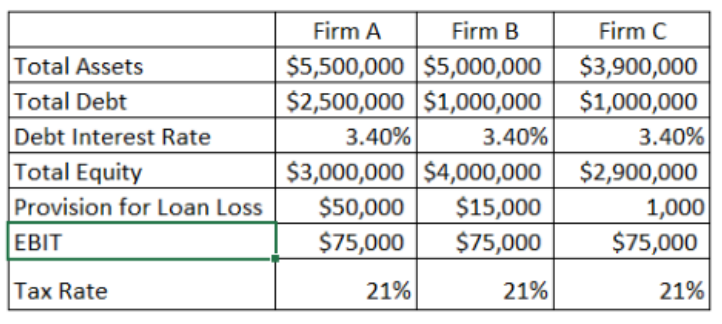
\includegraphics[width=0.6\textwidth]{2·17·1.png} 
      \end{figure}
      Given the above information, which firm has the higher return on equity (ROE)?
  \end{question}
  
  \begin{choices}
      \item Firm C has the highest ROE due to its lower equity position.
      \item Firm A had the higher ROE because of its large debt position.
      \item Without credit losses, firm A would have had the highest ROE.
      \item Without credit losses, firm B would have had the highest ROE.
  \end{choices}
  
  \begin{correctanswer}
      A
  \end{correctanswer}
  
  \begin{explanation}
      \textbf{A选项正确。} True: Firm C has the highest ROE due to its lower equity position.
      \begin{itemize}
          \item Firm A has a negative ROE ($-0.33\%$) because of its large debt position (as illustrated below). Even after sustaining credit losses the firm still must repay its debt holders. The A sustained heavy credit losses that lowered EBIT. However, even after adjusting for its credit losses Firm A still would have had a smaller ROE than firms B and C.
          \item Firm B had a positive ROE, but the ROE is very small because of its large equity compared to firms C and A. Firm A sustained a large credit loss that lowered EBIT. However, even after adjusting for its credit losses the firm would have still had a smaller ROE than firm C.
          \item Firm C had the highest ROE because of its small equity and modest credit loss.
      \end{itemize}
      \begin{figure}[H]
          \centering
          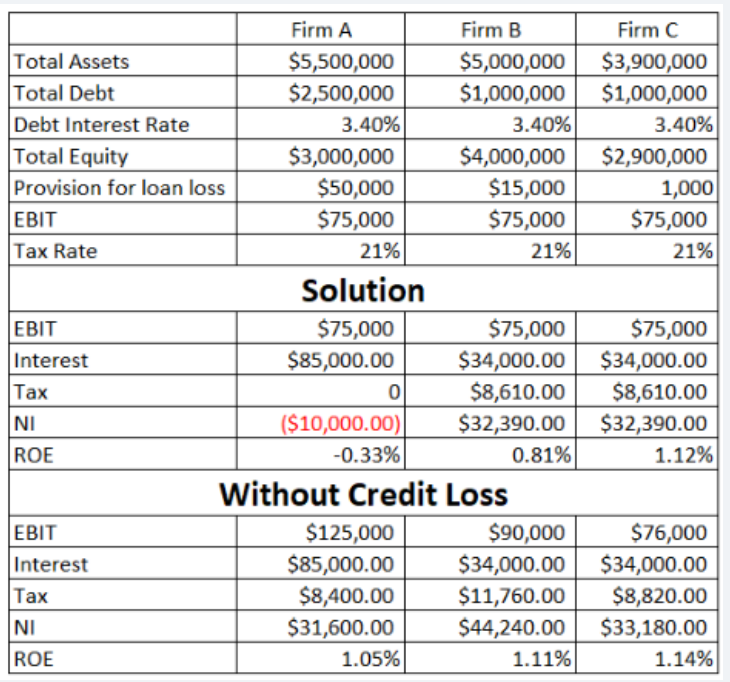
\includegraphics[width=0.6\textwidth]{2·17·2.png} 
      \end{figure}
  \end{explanation}
  
  \checklist{Finance: Financial Statement Analysis}{3}{2}
  
  % --- Question 18 ---
  \begin{question}
      The three lines of defense model (3LoD) has existed in some variation for over 30 years, although it achieved more visibility in 2013 when the Institute of Internal Auditors (IIA) published its initial position paper on the 3LoD, which it updated in 2021 (The IIA's Three Lines Model, an update of the Three Lines of Defense). GARP recommends firms refer to this update because the IIA ``has refined the model to reflect the evolution of risk management within organizations and aim to foster closer collaboration between business functions including internal audit.''
  
      In regard to the 3LoD model, each of the following is true EXCEPT which is false?
  \end{question}
  
  \begin{choices}
      \item The first line defines the organization's risk appetite but should not attempt to directly influence its risk culture
      \item The first line is responsible for implementing and maintaining effective controls to manage material operational risks
      \item The second line is part of management (and owns the ORM methodology) but provides support to the first line in order to help the firm create and protect value
      \item The third line has the clearest boundaries due to its independence
  \end{choices}
  
  \begin{correctanswer}
      A
  \end{correctanswer}
  
  \begin{explanation}
      \textbf{A选项正确。} A. False, both clauses. Instead, the following is true: The risk appetite (i.e., risk appetite statement) is developed by senior management and approved by the board. The risk culture is not the sole responsibility but is foundational to the firm's actual ORMF, such that all employees bear some responsibility for culture.
      
      In regard to (B), (C), and (D), each is TRUE.
  \end{explanation}
  
  \checklist{Operational Risk}{3}{2}
  
  % --- Question 19 ---
  \begin{question}
      Liquidity Early Warning Indicators (EWI) can be compared to an automobile's dashboard signal system where the appearance of a red light points our attention to something that may become a problem if not addressed. Each of the following is a credible red indicator (aka, red flag) in a Liquidity Early Warning Indicator (aka, Liquidity EWI) dashboard EXCEPT which is not a red (red flag) liquidity indicator?
  \end{question}
  
  \begin{choices}
      \item Narrowing debt/CDS spreads
      \item Sudden increase in debt costs
      \item Sudden growth in assets accompanied by volatile liabilities
      \item Rapid decline in the weighted average maturity of liabilities
  \end{choices}
  
  \begin{correctanswer}
      A
  \end{correctanswer}
  
  \begin{explanation}
      \textbf{A选项正确。} A. FALSE. Instead, the liquidity EWI is: a widening debt/CDS spreads (consistent with a sudden increase in debt costs)
      
      In regard to (B), (C), and (D), each is a candidate Liquidity EWI, per the Study Note:
      ``The Basel Committee on Banking Supervision (BCBS) recommends certain measures as EWI. These measures include [collapsed here, new emphasis ours]:
      \begin{itemize}
          \item An unusual growth in assets, particularly when accompanied by volatile liabilities;
          \item Debt (credit) spreads \textit{widen}, and/or credit default swap (CDS) spreads \textit{widen}.
          \item Declining diversity in the makeup of assets and liabilities; Growing currency mismatches;
          \item When the weighted average of liabilities' maturity declines;
          \item Positions going beyond or getting close to regulatory limits;
          \item Certain product line experience negative trends; The financial condition of the bank weakens; Public press that is negative;
          \item A downgrade in the credit rating; A decline in the stock price;
          \item Debt costs increase; Retail and/or wholesale funding costs increase;
          \item Counterparties becoming nervous about the financial condition of the bank;
          \item Credit lines are lowered;
          \item Outflows of retail deposits at an increased pace; Certificates of deposit (CDs) are increasingly redeemed;
          \item Longer-term funding opportunities become more difficult; and Placing short-term liabilities becomes more difficult''
      \end{itemize}
  \end{explanation}
  
  \checklist{Liquidity Risk Management}{3}{2}
  
  % --- Question 20 ---
  \begin{question}
      In factor theory, an asset's risk premium (aka, expected excess return) is given by $E(r_i) - R_f = \beta(i,m) \times \lambda(m)$ where the asset's beta is with respect to the stochastic discount factor (SDF; aka, pricing kernel) and $(m)$ in an index of bad time. Let’s make the following assumptions about an asset:
      \begin{itemize}
          \item The riskfree rate is $3.0\%$ such that $E(m) = 1/1.03 = 0.9709$
          \item The variance$(m)$ equals $30.0\%^2 = 0.090$
          \item The covariance$(r_i, m)$ equals $-0.10680$
      \end{itemize}
      Which is \textbf{nearest} to the asset's risk premium which refers to the asset's expected excess return, $E(r_i) - R_f$?
  \end{question}
  
  \begin{choices}
      \item -5.0\%
      \item +4.0\%
      \item +8.0\%
      \item +11.0\%
  \end{choices}
  
  \begin{correctanswer}
      D
  \end{correctanswer}
  
  \begin{explanation}
      \textbf{D选项正确。} The expected excess return, $E(r_i) - R_f = \beta(i,m) \times \lambda(m)$ where $\beta(i,m) = \text{cov}(r_i, m)/\text{var}(m)$ and $\lambda(m) = -\text{var}(m)/E(m)$.
      
      In this case, $\beta(i,m) = \text{cov}(r_i, m)/\text{var}(m) = -0.10680/0.090 = -1.186667$, and $\lambda(m) = -\text{var}(m)/E(m) = -0.090/0.9709 = -0.0926975$.
      
      Therefore, $E(r_i) - R_f = \beta(i,m) \times \lambda(m) = -1.186667 \times -0.0926975 = 0.1100011$ or about $11.0\%$.
  \end{explanation}
  
  \checklist{Finance: Factor Theory}{3}{2}
  
  % --- Question 21 ---
  \begin{question}
      Below (in the left-hand panel) is an interest rate tree for the one-year rate where the initial rate of $8.0\%$ jumps 300 basis points to either $11.0\%$ or $5.0\%$ next year. In two years, the one-year rate will be either $2.0\%$, $8.0\%$, or $14.0\%$.
  
      Next, we will assume a three-year zero-coupon bond. Without a risk premium, for example, the date 0, state 2 price would be $0.877193 = 1/(1+14\%)$. However, we will instead assume a risk premium. Specifically, investors require compensation of 50 basis points for each year of duration risk. The right-hand panel displays the associated risk-neutral (i.e., , assumes the risk premium) price tree for this three-year zero-coupon bond
  
      \begin{figure}[H]
          \centering
          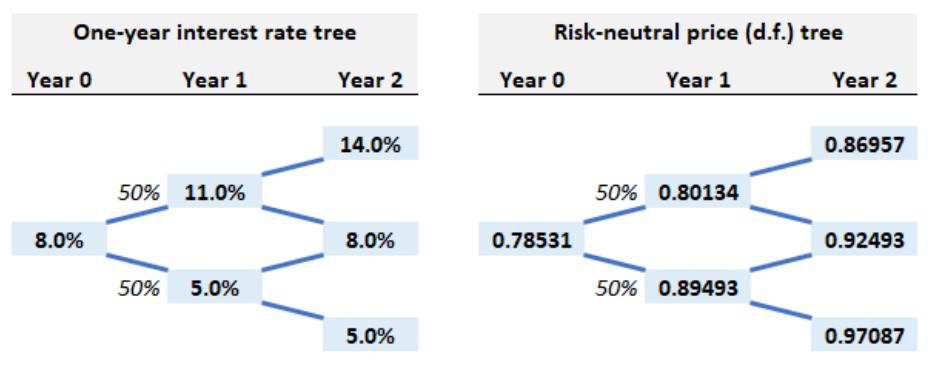
\includegraphics[width=0.48\textwidth]{2·21.png}
      \end{figure}
  
      In regard to the three-year zero-coupon bond, which of the following is true?
  \end{question}
  
  \begin{choices}
      \item The expected return over the next year is $7.50\%$
      \item The expected return over the next year is $9.00\%$
      \item The implied 3-year spot rate term structure is downward sloping (aka, inverted)
      \item Jensen's inequality implies that expected excess return over two years is less than 50 basis points
  \end{choices}
  
  \begin{correctanswer}
      B
  \end{correctanswer}
  
  \begin{explanation}
      \textbf{B选项正确。} True: The expected return over the next year is $9.00\%$.
  
      We don’t require the formula. The risk premium is 50 basis points for each year of duration risk, and the three-year bond creates two years of duration risk. The expected return, therefore, is 100 basis points above $8.0\%$.
  \end{explanation}
  
  \checklist{Fixed Income}{3}{2}
  
  % --- Question 22 ---
  \begin{question}
      Old Crow Bank had a credit committee meeting yesterday, and the following is a copy of the notes taken during the meeting:
      \begin{itemize}
          \item All members are present Jan (Chief Risk Officer), Eddie (Head of Compliance), Alyssa (Head of Legal), Don (Head of Tax), and Ashton (Chief Financial Officer).
          \item Jan initiated the meeting by confirming if everyone had received an email containing approval documents from credit officer Doug, who had originated the loan. Everyone confirmed receiving the email with the documents yesterday.
          \item Jan provided an overview of the loan for approximately five minutes, after which she proceeded to inquire about the opinions of those present. It was the consensus of all individuals, except for Alyssa, that the loan be approved. Alyssa expressed concern regarding the trustworthiness of the counterparty.
          \item Jan respects Alyssa’s opinion but disagrees and initiates a vote. Two other committee members agree with Jan, resulting in loan approval.
      \end{itemize}
      What is the most probable issue with the credit committee’s meeting?
  \end{question}
  
  \begin{choices}
      \item The approval documents should have been distributed earlier.
      \item Jan monopolized the conversation and did not properly facilitate discussion.
      \item The meeting was not properly documented.
      \item The vote was not unanimous, so the loan should have been rejected.
  \end{choices}
  
  \begin{correctanswer}
      C
  \end{correctanswer}
  
  \begin{explanation}
      \textbf{Option C is correct.} In this scenario, all the approval documents were appropriately distributed to the committee before the meeting. Jan did spend time explaining the investment to the committee, but she also helped facilitate discussion among the committee members and listened to everyone’s opinion. Votes do not have to be unanimous, but they should be held unless the decision is unanimous. However, meetings should be accurately documented in case an investment goes awry. In the case of a bad transaction, auditors would want to know what was discussed in the meeting and if the reasoning is behind the investment decision.
  \end{explanation}
  
  \checklist{Credit Risk Management}{3}{2}
  
  % --- Question 23 ---
  \begin{question}
      A bank is using the VaR and stressed VaR (SVaR) market risk framework according to the Basel 2.5 guidelines. The bank’s internal models for market risk have generated the following risk measures for the current trading book positions (VaR and SVaR are in USD millions):
      \begin{figure}[H]
          \centering
          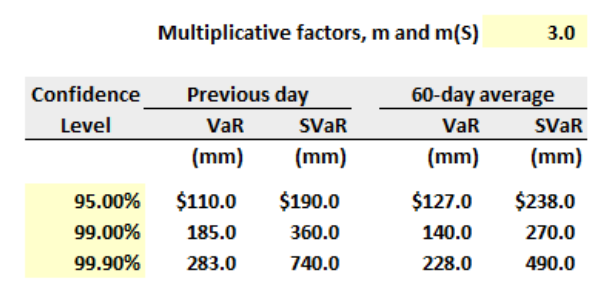
\includegraphics[width=0.6\textwidth]{2·23.png} 
      \end{figure}
      The supervisor has set both multiplication factors, m and m(S), to 3.0. What is the correct capital requirement for general market risk for the bank under Basel 2.5? (note: this question inspired by Question 42 of GARP’s 2020 Part 2 Practice Exam).
  \end{question}
      
      \begin{choices}
          \item \$630.0 million
          \item \$810.0 million
          \item \$1,230.0 million
          \item \$2,154.0 million
      \end{choices}
      
      \begin{correctanswer}
      C
      \end{correctanswer}
      
      \begin{explanation}
      \textbf{C选项正确。} True: \$1,230.0 million
      
      The Basel 2.5 market risk capital requirement requires a 99.0\% confidence level and is given by: 
      \[ MRC = \max[VaR(t-1), m \times VaR(60\text{-day avg})] + \max[SVaR(t-1), m(S) \times SVaR(60\text{-day avg})] \]
      In this case, 
      \[ MRC = \max[185.0, 3.0 \times 140.0] + \max[360.0, 3.0 \times 270.0] = \$1,230.0 \text{ million}. \]
      \end{explanation}
      
  \checklist{Market Risk}{3}{2}
  
  % --- Question 24 ---
  \begin{question}
      If a corporation's marginal tax rate is $30.0\%$ and it purchases an A-rated municipal bond that offers a $4.20\%$ gross yield (aka, yield to maturity), what is the tax equivalent yield (TEY)?
  \end{question}
  
  \begin{choices}
      \item $2.45\%$
      \item $3.50\%$
      \item $6.00\%$
      \item $16.67\%$
  \end{choices}
  
  \begin{correctanswer}
  C
  \end{correctanswer}
  
  \begin{explanation}
      \textbf{C选项正确。} TRUE: $6.00\%$. $\text{TEY} = \text{after-tax return on tax-exempt investment} / (1 - \text{marginal tax rate})$; in this case, $\text{TEY} = 4.20\%/(1 - 0.30) = 6.00\%$
  \end{explanation}
  
  \checklist{Finance: Fixed Income}{1}{1}
  
  % --- Question 25 ---
  \begin{question}
      Andrew Ang introduces factors and divides them primarily into two types: macro, fundamental-based factors \underline{versus} investment-style factors. He writes, ``Factors drive risk premiums. One set of factors describes fundamental, economywide variables like growth, inflation, volatility, productivity, and demographic risk. Another set consists of tradeable investment styles like the market portfolio, value-growth investing, and momentum investing.'' ($\dagger$)
  
      Ang also claims that the three most important macro factors are growth, inflation, and volatility. His evaluation of these macro factors is based on a long-term historical sample (specifically, 1952:Q1 to 2011:Q4). It is important to qualify the sample window because we cannot be sure that past is prologue; e.g., interest rates experienced two long-term secular trends during this window.
  
      In regard to his historical analysis, each of the following statements is true EXCEPT which is false?
  \end{question}
  
  \begin{choices}
      \item Government and investment-grade bonds performed BETTER during economic recessions than during expansions
      \item Both large and small (cap) stocks perform significantly BETTER during economic expansions than during recessions
      \item During periods of high inflation, all five asset classes perform significantly BETTER than during periods of low inflation
      \item All five assets classes are much MORE VOLATILE during recessions (or periods of low GDP growth) than during expansions
  \end{choices}
  
  \begin{correctanswer}
      C
  \end{correctanswer}
  
  \begin{explanation}
      \textbf{C选项正确。} False. To be true, this should instead read: During periods of high inflation, all five asset classes perform significantly WORSE than during periods of low inflation.
      
      In regard to (A), (B) and (D), each is TRUE.
  \end{explanation}
  
  \checklist{Factor Investing}{3}{3}
  
  % --- Question 26 ---
  \begin{question}
      Below is the price tree for a stylized constant-maturity Treasury (CMT) swap struck at 2.0\% with a notional of \$1.0 million. The risk-neutral probabilities are displayed, specifically: 80.09\% (d = 19.91\%) from date 0 to date 1; and 65.20\% (d = 34.80\%) from date 1 to date 2. Using these risk-neutral probabilities returns an expected discounted value (EDV) of \$3,702.11 for the value of the CMT swap. Please notice this exactly matches Tuckman's Figure 7.8 in his 4th edition value. This is the so-called model value.
  
      \begin{figure}[H]
          \centering
          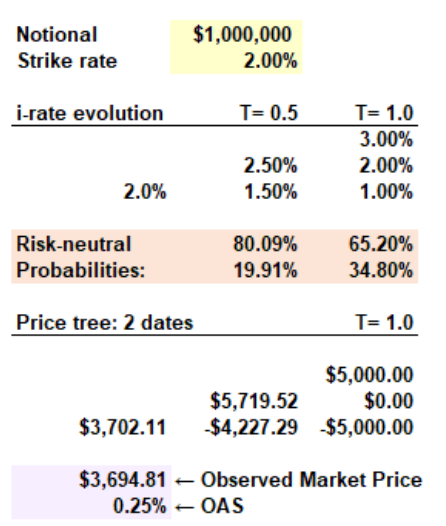
\includegraphics[width=0.6\textwidth]{2·26.png} 
      \end{figure}
  
      Assume the observed market price of this CMT swap is \$3,694.81 (as highlighted in purple), which is \$7.30 less than the market price. This implies an option-adjusted spread (OAS) of 25 basis points. Which of the following is the \textbf{best} interpretation of this OAS?
  \end{question}
  
  \begin{choices}
      \item The model returns the market price if we adjust the risk-neutral probabilities to 55.09\% and 44.91\%
      \item The model returns the market price if we assume adjusted cash flows; e.g., \$3,750 instead of \$5,000 on (state 2, date 2)
      \item The model returns the market price if we use discount rates of 2.25\% (date 0, state 0), 1.75\% (date 1, state 0), and 2.75\% (date 1, state 1)
      \item We cannot interpret the OAS here because this is a CMT swap, and the OAS requires an embedded option; e.g., a bond with an embedded call option
  \end{choices}
  
  \begin{correctanswer}
  C
  \end{correctanswer}
  
  \begin{explanation}
      \textbf{C选项正确。} True: The model returns the market price if we use discount rates of 2.25\% (date 0, state 0), 1.75\% (date 1, state 0), and 2.75\% (date 1, state 1)
  \end{explanation}
  
  \checklist{Fixed Income Analysis}{3}{2}
  
  % --- Question 27 ---
  \begin{question}
      Strongcore Financial Corporation has purchased a long-term at-the-money (ATM) call option from a risky counterparty. The option’s stock and strike price are \$25.00 million. The underlying asset’s volatility, $\sigma$, is estimated to be 20.0\% while the risk-free rate is 3.0\% per annum. The European-style option matures in 3.0 years. In regard to the standard normal cumulative distribution function, in this scenario $N(d1)$ equals 0.66750 and $N(d2)$ equals 0.53450.
  
      With respect to its counterparty risk, Strongcore assigns a hazard rate estimate of 6.0\% and believes its counterparty could default at any time during the three-year option period; i.e., the cumulative default probability is relevant for this approximation. Further, if its counterparty defaults, Strongcore assigns a conservative recovery rate estimate of 30.0\%.
  
      In summary, the assumptions are: $S = K = \$25.0$ million, $\sigma = 20.0\%$, $R_f = 3.0\%$, $T = 3.0$ years; $\lambda$ (i.e., hazard rate) = 6.0\%, and $LGD = 70.0\%$.
  
      In this situation, Strongcore does NOT want to compute the standard credit value adjustment (CVA) formula which is the summation of discounted expected exposures, $EE(t)$, over multiple future periods. Instead, Strongcore wants to rely on the simpler ``semi-analytical method'' that produces an estimate as a function of the position’s current value, the cumulative default probability, $PD(0,T)$, and the loss given default, $LGD$. Under this simpler approximation, which of the following is \textbf{nearest} to the CVA charge for the long option position?
  \end{question}
  
  \begin{choices}
      \item \$15,600
      \item \$90,000
      \item \$516,000
      \item \$1.1 million
  \end{choices}
  
  \begin{correctanswer}
      C
  \end{correctanswer}
  
  \begin{explanation}
      \textbf{C选项正确。} \$516,000
      
      $CVA = -LGD \times PD(0,T) \times V(t)$. In this case, $V(t) = S \times N(d1) - K \times \exp(-rt) \times N(d2) = 25 \times 0.66750 - 25 \times \exp(-0.030 \times 3) \times 0.53450 = \$4.475$ million. The cumulative $PD = 1 - \exp(-0.060 \times 3) = 16.473\%$. Therefore the CVA approximation is given by $70\% \times 16.473\% \times 4.475 \text{ million} = \$0.5160 \text{ million}$, or \$516,002.
  \end{explanation}
  
  \checklist{Credit Risk}{27}{2}
  
  % --- Question 28 ---
  \begin{question}
      Andrew is preparing to make a presentation to the board. The presentation’s goal is to introduce a new, proposed operational risk management (ORM) framework and get the board’s feedback on the way to eventual approval. It happens to be the case that his company is publicly traded with a high cost of capital due to its above-average beta.
  
      The board members are generally more familiar with market and credit risk but less familiar with operational risk. Therefore, his presentation will review several of the features (and nature) of operational risk, including its dynamic evolution. His presentation will briefly explore the skewed, heavy-tailed feature of operational risk. For candidate frequency distributions, he will illustrate the Poisson and negative binomial. For candidate severity distributions, he will illustrate the log-normal and generalized Pareto Distribution (GPD).
  
      In addition to these features (i.e., dynamic, heavy-tailed), which of the following is TRUE about operational risk?
  \end{question}
  
  \begin{choices}
      \item The easiest way for a high-beta firm to lower its beta is to centralize the operational risk management (ORM) function
      \item Operational risk is highly homogeneous because so-called boundary events define clusters that contain loss events and their shared (aka, common) features
      \item ORM is valuable because it reduces regulatory capital, and regulatory capital is a good indicator of the firm's quality of risk management
      \item Most causes of operational risk trace to control weaknesses; human biases and behavioral failings; and/or operating environment changes
  \end{choices}
  
  \begin{correctanswer}
      D
  \end{correctanswer}
  
  \begin{explanation}
      \textbf{Option D is correct.} Most operational risk causes trace to control weaknesses; human biases and behavioral failings; and/or operating environment changes
  
      In regard to (A), (B), and (C), each is FALSE.
      \begin{itemize}
          \item Operational risk is predominantly idiosyncratic and diffuses within the firm. Beta is a systematic risk.
          \item Operational risk is highly heterogeneous but interconnected. Further, boundary events are “risk events that materialize in a different category than they cause” –Source: GARP Introduction to Operational Risk and Resilience, Section 1.5)
          \item According to GARP, “regulatory operational risk capital is not sensitive enough to a firm’s risk profile and thus brings no real incentive to optimize the management of operational risks. In fact, regulatory capital is often a poor indicator of risk management quality.” –Source: Chapter (GARP Introduction to Operational Risk and Resilience, Section 1.7)
      \end{itemize}
  \end{explanation}
  
  \checklist{Operational Risk}{3}{2}
  
  % --- Question 29 ---
  \begin{question}
      Over the next 24 hours, Greenlux State Bank estimates that the following cash inflows and outflows (all figures in millions) will occur:
      \begin{figure}[H]
          \centering
          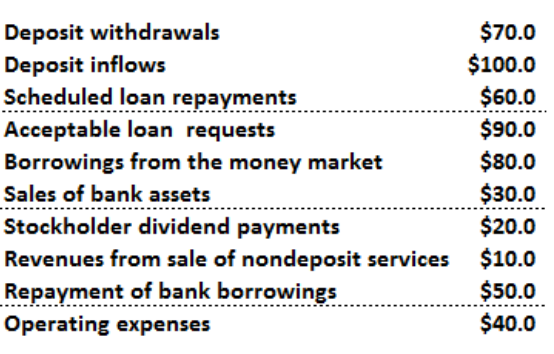
\includegraphics[width=0.6\textwidth]{2·29.png} 
      \end{figure}
      What is the bank's projected net liquidity position?
  \end{question}
  
  \begin{choices}
      \item -30.0 million
      \item +10.0 million
      \item +40.0 million
      \item +90.0 million
  \end{choices}
  
  \begin{correctanswer}
      B
  \end{correctanswer}
  
  \begin{explanation}
      \textbf{B. TRUE: +10.0 million}
      
      Inflows include:
      Deposit inflows = $100 +$
      Scheduled loan repayments = $60 +$
      Borrowings from the money market = $80 +$
      Sales of bank assets = $30 +$
      Revenues from sale of nondeposit services = $10$;
      for total inflows of $\$100 + \$60 + \$80 + \$30 + \$10 = 280.0$ million.
      
      Outflows include:
      Deposit withdrawals = $70 +$
      Acceptable loan requests = $90 +$
      Stockholder dividend payments = $20 +$
      Repayment of bank borrowings = $50 +$
      Operating expenses = $40$;
      for total outflows of $\$70 + \$90 + \$20 + \$50 + \$40 = \$270.0$ million
      
      Therefore, the projected net liquidity position = $\$280 - 270 = +10.0$ million.
  \end{explanation}
  
  \checklist{Finance}{3}{2}
  
  % --- Question 30 ---
  \begin{question}
      Emily manages a $\$20.0$ million portfolio allocated into two positions (aka, two components): a Technology ETF, and a Real Estate Investment Trust (REIT) ETF. She compares four different allocations, where the weight assigned to the Tech ETF component is either $35.0\%$, $50.0\%$, $65\%$, or $80.0\%$.
  
      \begin{figure}[H]
          \centering
          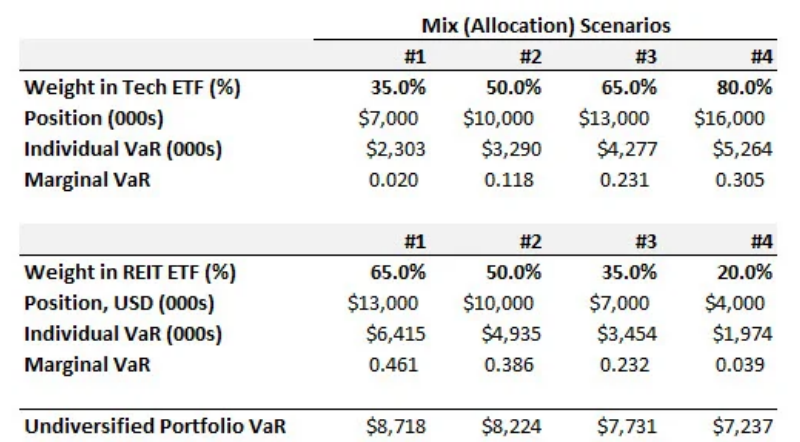
\includegraphics[width=0.6\textwidth]{2·30.png} 
      \end{figure}
  
      If her goal is to minimize the portfolio’s diversified value at risk (VaR), which of the above allocations is \textbf{best}?
  \end{question}
  
  \begin{choices}
      \item Mix \#1 with $35.0\%$ allocated to the Tech ETF
      \item Mix \#2 with $50.0\%$ allocated to the Tech ETF
      \item Mix \#3 with $65.0\%$ allocated to the Tech ETF
      \item Mix \#4 with $80.0\%$ allocated to the Tech ETF
  \end{choices}
  
  \begin{correctanswer}
  C
  \end{correctanswer}
  
  \begin{explanation}
      \textbf{Option C is correct.} Mix \#3 with $65.0\%$ allocated to the Tech ETF.
      
      Risk is minimized (i.e., the portfolio’s diversified VaR is minimized) when the marginal VaRs are constant. Among the four mixes, mix \#3 is clearly the choice where the marginal VaRs are nearest (i.e., $0.231$ versus $0.232$ is almost an exact match). Mix \#1 has the greatest diversified VaR. Starting from Mix \#1, risk is reduced by ADDING to the component with the lower marginal VaR (in this mix, the marginal VaR of the Tech ETF is only $0.020$ while the marginal VaR of the REIT ETF is $0.461$) and REDUCING the component with the higher marginal VaR. If we thusly start with Mix \#1 and add $15.0\%$ to the Tech ETF, then we “arrive” at Mix \#2. However, in Mix \#2 the Marginal VaR of the REIT ETF is still much higher than the Marginal VaR of the Tech ETF (i.e., $0.386$ versus $0.118$) so we can continue to shift toward the position with the lower Marginal VaR (which is still the Tech ETF). If we add another $15\%$ to the Tech ETF, then we arrive at Mix \#3: here the Marginal VaRs are almost equal, so we are very close to the allocation that minimizes the portfolio’s diversified VaR. For the record, the diversified portfolio VaR for the four mixes are $\$6,131.14$ (Mix \#1), $\$5,043.03$ (Mix \#2), $\$4,621.42$ (Mix \#3), and $\$5,036.58$ (Mix \#4).
  \end{explanation}
  
  \checklist{Finance: Risk Management}{3}{2}
  
  % --- Question 31 ---
  \begin{question}
      In comparison to a yield-based DV01 hedge, which of the following is the \textbf{best} argument in favor of a regression hedge?
  \end{question}
  
  \begin{choices}
      \item The regression hedge minimizes the profit and loss (P\&L) variance of the hedged position
      \item The regression hedge is based on economic theory and future developments rather than empirical analysis
      \item The regression hedge does not require any out-of-sample test(s), which are often unreliable if the sample is small
      \item The regression hedge solves for a risk-weight which qualifies as a valid risk-weighted asset (RWA) under Basel regulations
  \end{choices}
  
  \begin{correctanswer}
      A
  \end{correctanswer}
  
  \begin{explanation}
      \textbf{A选项正确。} True: The regression hedge minimizes the profit and loss (P\&L) variance of the hedged position.
      
      As Tuckman explains (emphasis ours), “The \textbf{best argument for the regression hedge} is actually not the earlier assumption that bond yields change exactly according to the regression model. Write the P\&L of the position as ... formula 6.11 ... where the negative signs reflect that a positive face amount with a positive change (i.e., increase) in yield lowers P\&L. It can then be shown that the regression hedge in Equation (6.8) minimizes the variance. In other words, \textbf{to the extent that P\&L variance is an appropriate measure of risk, the regression hedge minimizes the risk of the hedged position.}” –Tuckman, Bruce; Serrat, Angel. Fixed Income Securities (Wiley Finance) (p. 159). Wiley. Kindle Edition.
      
      In regard to (B), (C), and (D), each is FALSE. Instead, the following are true statements:
      \begin{itemize}
          \item The regression hedge is based on empirical analysis but not economic theory and future developments
          \item The regression hedge typically does require (or at least prefer) out-of-sample test(s)
          \item The risk weight is the beta coefficient and has nothing to do with risk-weighted asset (RWA) under Basel regulations
      \end{itemize}
  \end{explanation}
  
  \checklist{Fixed Income: Hedging}{3}{2}
  
  % --- Question 32 ---
  \begin{question}
      Among its financial positions, Zapex Financial Corporation has written a call, entered into an interest rate swap, and written a credit default swap. Among these (the following) four positions, which is the BEST example of wrong-way risk?
  \end{question}
  
  \begin{choices}
      \item Zapex has written (aka, sold) a call option to a counterparty in the same industry
      \item Zapex is the fixed-rate payer in an interest rate swap during an economic recovery
      \item Zapex has written (aka, sold) a credit default swap (CDS) to counterparty whose credit quality is positively correlated with the reference entity
      \item Zapex has a position in a forward currency contract where its mark-to-market gain is positively correlated with the counterparty's default probability
  \end{choices}
  
  \begin{correctanswer}
      D
  \end{correctanswer}
  
  \begin{explanation}
      \textbf{D选项正确。} Zapex has a position in a forward currency contract where its mark-to-market gain is positively correlated with the counterparty's default probability
      
      Wrong-way (credit) risk is adverse correlation between the exposure and the credit quality, so wrong-way risk is a positive (negative) correlation between exposure and default probability (credit quality). This is wrong-way risk because greater exposure is associated with a lower likelihood of payment. Algebraically, wrong-way (or right-way) risk is some dependence between exposure/EAD and PD. We normally write $EL\% = PD \times EAD$ but that assumes independence between PD and EAD, so a way to think about WWR is simply when $EL > PD \times EAD$, because $EL \neq PD \times EAD$ is also a condition for non-independence.
      
      In regard to (A), (B) and (C), each is an example of RIGHT-WAY risk.
  \end{explanation}
  
  \checklist{Credit Risk: Wrong-Way Risk}{3}{2}
  
  % --- Question 33 ---
  \begin{question}
      According to the FDIC, model risk management starts with robust model development, implementation, and use (aka, the first element. The second element is a sound validation process. The third element is governance). Which of the following is a TRUE statement about this \textit{first element} (development, implementation and use) of model risk management?
  \end{question}
  
  \begin{choices}
      \item Model development should be a straightforward and routine technical process
      \item To exercise conservatism, pick an extreme point on a given modeled distribution
      \item Banks should never model output with judgmental or qualitative adjustments
      \item Although the nature of testing varies by the context and type of model, testing is an integral part of model development
  \end{choices}
  
  \begin{correctanswer}
      D
  \end{correctanswer}
  
  \begin{explanation}
      \textbf{D. TRUE:} Although the nature of testing varies by the context and type of model, testing is an integral part of model development
      
      In regard to (A), (B) and (C), each is FALSE.
      \begin{itemize}
          \item Model development is neither straightforward nor a routine technical process!
          \item To pick an extreme point on a given modeled distribution is not necessarily conservative if the distribution is mis-specified or mis-estimated in the first place.
          \item Judgmental or qualitative adjustments are a KEY part of model development/implementation/use: ``In addition, a considerable amount of subjective judgment is exercised at various stages of model development, implementation, use, and validation. It is important for decision makers to recognize that this subjectivity elevates the importance of sound and comprehensive model risk management processes.'' ... ``Banks should ensure that the development of the more judgmental and qualitative aspects of their models is also sound. In some cases, banks may take statistical output from a model and modify it with judgmental or qualitative adjustments as part of model development.''
      \end{itemize}
  \end{explanation}
  
  \checklist{Operational Risk: Model Risk Management}{3}{2}
  
  % --- Question 34 ---
  \begin{question}
      Suppose that Acme Bank reports interest-sensitive assets (ISA) of \$490.0 million and interest-sensitive liabilities (ISL) of \$610.0 million. Recall that the relative interest-sensitive gap (aka, Relative IS GAP) is equal to the Dollar IS GAP divided (aka, scaled) by the size of the bank (where IS assets is a valid measure of size). Respectively, what is the bank’s relative IS GAP; its interest-sensitivity ratio (ISR); and the impact of rising interest rates on its net interest margin (NIM)?
  \end{question}
  
  \begin{choices}
      \item The Relative IS GAP is -120.0; the ISR is 1.245; rising interest rates will lower the NIM
      \item The Relative IS GAP is -0.245; the ISR is 0.803; rising interest rates will lower the NIM
      \item The Relative IS GAP is -0.245; the ISR is 1.245; rising interest rates will increase the NIM
      \item The Relative IS GAP is +4.08; the ISR is 0.803; rising interest rates will increase the NIM
  \end{choices}
  
  \begin{correctanswer}
      B
  \end{correctanswer}
  
  \begin{explanation}
      \textbf{B选项正确。} The Dollar IS GAP = ISA – ISL = $\$490.0 - \$610.0 = -120.0$. The Relative IS GAP = $-120.0/490.0 = -0.245$. The ISR = $490.0/610.0 = 0.803$. This bank is liability-sensitive such that rising interest rates will lower its net interest margin (NIM).
  \end{explanation}
  
  \checklist{Market Risk: Interest Rate Risk}{3}{2}
  
  % --- Question 35 ---
  \begin{question}
      You work for the Private Client division of an international bank. The bank's Private Client Advisors work with high net worth (NNW) individuals and families. Your boss has tasked you to perform due diligence on a roster of hedge funds; the funds that survive your due diligence will become candidates for presentation (and recommendation) to suitable customers of the bank who will become investors in the fund(s).
  
      Your boss says that your due diligence should include a careful screen for fraud risk on behalf of the investors. In the case of your due diligence, which of the following is the most important ingredient?
  \end{question}
  
  \begin{choices}
      \item Diligent application of a comprehensive checklist including a list of specific questions
      \item Strong pre-existing personal relationships among the fund's managers and all related parties
      \item Guarantees by the fund of exceptional performance (e.g., $>30\%$ per annum) with little or no risk
      \item The investors' membership in an affinity group, preferably a religious group due to high correlation with ethics
  \end{choices}
  
  \begin{correctanswer}
      A
  \end{correctanswer}
  
  \begin{explanation}
      \textbf{A. TRUE:} Diligent application of a comprehensive checklist including a list of specific questions
      
      The authors recommend reviewing the SEC website including its list of questions; e.g., Red Flags of Investment Fraud Checklist at https://www.investor.gov/.
      
      In regard to (B), (C) and (D), each is false:
      \begin{itemize}
          \item Strong pre-existing personal relationships with related parties is the \textbf{opposite of the independence} that investors should require between fund managers and related parties.
          \item Guarantees of exceptional performance with little or no risk is a classic \textbf{red flag}.
          \item In regard to affinity groups: these are notorious targets of fraud because participants tend to be trusting of their peers.
      \end{itemize}
  \end{explanation}
  
  \checklist{Finance: Due Diligence}{35}{4}
  
  % --- Question 36 ---
  \begin{question}
      Which of the following is the BEST summary of the purpose of a copula function?
  \end{question}
  
  \begin{choices}
      \item To utilize the Gaussian correlation matrix such that tractable pairwise correlation parameters replace intractable dependence values
      \item To specify a single multivariate distribution as a function of various (even unusual) univariate marginal distributions by mapping them to distributions with an accessible or familiar dependence structure
      \item To translate a vector of outcomes into quantiles and map the quantiles to probabilities such that virtually any combination of multiple outcomes can be expressed as a single vector
      \item To decompose a posterior conditional distribution into a combination of the prior probability, the likelihood, and the marginal probability, typically by identifying Cholesky's decomposition
  \end{choices}
  
  \begin{correctanswer}
  B
  \end{correctanswer}
  
  \begin{explanation}
      \textbf{B选项正确。} To specify a single multivariate distribution as a function of various (even unusual) univariate marginal distributions by mapping them to distributions with an accessible or familiar dependence structure
  \end{explanation}
  
  \checklist{Quantitative Analysis: Copulas}{1}{1}
  
  % --- Question 37 ---
  \begin{question}
      Retail exposures include the following: credit cards, installment loans (e.g., personal finance, educational loans, auto loans, leasing), revolving credits (e.g., overdrafts, home equity lines of credit), and residential mortgages. Each of the following tends to be a stronger feature of retail credit risk rather than corporate credit risk EXCEPT which is more typical of corporate credit risk?
  \end{question}
  
  \begin{choices}
      \item Portfolio tends to behave like a well-diversified portfolio in normal markets
      \item Default by a single customer is never expensive enough to threaten a bank
      \item A rise in defaults is often signaled in advance by a change in customer behavior
      \item Portfolio risk is dominated by risk that credit losses will rise to unexpected level due to concentrations of exposures
  \end{choices}
  
  \begin{correctanswer}
      D
  \end{correctanswer}
  
  \begin{explanation}
      \textbf{D选项正确。} This tends to be a feature of CORPORATE credit risk: portfolio risk is dominated by risk that credit losses will rise to unexpected level due to concentrations of exposures.
      \begin{itemize}
          \item In regard to (A), (B) and (C), each is a tendency of retail credit risk.
      \end{itemize}
  \end{explanation}
  
  \checklist{Credit Risk: Retail vs Corporate}{3}{2}
  
  % --- Question 38 ---
  \begin{question}
      According to the Basel Committee on Banking Supervision (BCBS, 2018), in regard to cyber-security and cyber-resilience metrics, “Some jurisdictions have methodologies to assess or benchmark regulated institutions’ cyber-security and resilience ... None of these methodologies produce quantitative metrics or risk indicators comparable to those available for financial risks and resilience; e.g., standardized quantitative metrics where established data are available. Instead, indicators provide information on regulated institutions’ approach to building and ensuring cyber-security and resilience more broadly. Supervisory authorities also rely on entities’ own management information, although this differs across entities and is not yet mature.”($\dagger$)
  
      With respect to current cybersecurity and resilience metrics, each of the following statements is true EXCEPT which is inaccurate?
  \end{question}
  
  \begin{choices}
      \item No single cybersecurity/resilience metric in isolation is sufficient
      \item Patch aging (aka, days to patch) is a widespread and comparable metric
      \item Backward-looking metrics are helpful but insufficient; forward-looking metrics are necessary because adversaries dynamically adapt
      \item The penetration ratio (i.e., percentage of banks in a jurisdiction that can be penetrated) is a useful metric that compares a supervisor's effectiveness to other jurisdictions
  \end{choices}
  
  \begin{correctanswer}
      D
  \end{correctanswer}
  
  \begin{explanation}
      \textbf{D选项正确。} False. The displayed penetration ratio is nonsensical (also to compare supervisor effectiveness), but penetration tests (penetration testing) are discussed several times by BCBS as an effective cyber-risk control approach. However, please do note that penetration testing (by type: count and finding rating) is a common and effective cyber-resilience metric. See 4.2.2. Penetration testing.
  
      In regard to (A), (B) and (C), each is TRUE. Specifically:
      \begin{itemize}
          \item No single cybersecurity/resilience metric in isolation is sufficient: “Collectively, these indicators [i.e., cyber-metrics collated by regulated entities] can inform on the broad adequacy of an institution’s cyber- and operational resilience levels for its business needs and risk appetite. However, no single item taken in isolation is seen as a sufficient metric, and no standard set of indicators has been identified so far to provide a meaningful benchmark.”($\dagger$)
          \item Patch aging (aka, days to patch) is a widespread and comparable metric: “Annex C contains cyber-centric metrics collated by a sample set of regulated institutions for decision-making bodies (boards and board sub-committees). It is notable that the data provided typically allow for trend information so that the reviewer can assess if the situation is getting better or worse. Some metrics track compliance with internal policies while others measure inherent risk. Patch ageing in particular is a widespread and comparable metric.”($\dagger$)
          \item Backward-looking metrics are helpful but insufficient; forward-looking metrics are necessary because adversaries dynamically adapt: “Backward-looking indicators comment on past performance as an indicator of future performance, which is reasonable when institutions’ operations and risk environment are relatively stable over time and more or less independent from outside influences. However, cyber-risk frustrates this because adversaries are dynamic, themselves adapting to institutions’ responses and protective measures, sometimes changing their tactics and strategies even in the space of a single cyber-incident. Distributed denial of service (DDOS) incidents are a good example, where the volume and scale of disrupted internet traffic generated has increased significantly in the last two years and adversaries adapt their techniques in response to an institution’s defences. While backward-looking metrics continue to be important, jurisdictions are increasingly recognising the need for forward-looking indicators as direct and indirect metrics of resilience, indicating whether a regulated institution is likely to be more or less resilient in the event of a risk crystallising.”($\dagger$)
      \end{itemize}
  \end{explanation}
  
  \checklist{Operational Risk}{3}{2}
  
  % --- Question 39 ---
  \begin{question}
      Venkat explains that “all risk management frameworks start with a governance structure that defines the roles and responsibilities of various bank employees and committees in overseeing risk-related activities,” and effective governance includes the oversight of intraday liquidity risk. In regard to the governance structure of intraday liquidity risk management which of the following statements is TRUE?
  \end{question}
  
  \begin{choices}
      \item Intraday liquidity risk should be accepted as a cost of doing business
      \item Roles and responsibilities should be defined within the eight lines (i.e., two times four) of defense model
      \item PCS Systems should only be a source of funds; if PCS becomes a use of funds, then a yellow flag should be triggered
      \item Intraday liquidity risk should be incorporated in the risk taxonomy and is a component of risk self-assessment including settlement risks.
  \end{choices}
  
  \begin{correctanswer}
      D
  \end{correctanswer}
  
  \begin{explanation}
      \textbf{Option D is correct.} Intraday liquidity risk should be incorporated in the risk taxonomy and is a component of risk self-assessment including settlement risks.
      
      In regard to (A), (B) and (C), each is FALSE.
      \begin{itemize}
          \item Venkat($\dag$) explains that Active Risk Management is characteristic of the governance of intraday LRM: “Active risk management. In many institutions, intraday liquidity risk is accepted as a cost of doing business and is not as actively managed with the same level of rigor as other types of enterprise risk or even other liquidity risks. The leading banks with large volumes of PCS activities recognize the criticality of understanding and working to reduce their intraday liquidity risks. These institutions classify settlement and systemic risks as components of their risk taxonomy, and critically, incorporate them into the firm’s risk appetite framework”($\dag$)
          \item Integration with risk governance includes the THREE lines of defense model: Treasure, Corporate Risk Management, and Internal Audit. Says Venkat($\dag$), “The intraday liquidity risk management framework follows the industry’s three lines of defense model, with particular emphasis on expertise in the second line of defense to coordinate across the institution ... Corporate Risk Management is the second line of defense, responsible for overseeing funding-related policy and procedures: advising in the development of risk management programs, monitoring the ongoing risk-taking activities across all of a bank’s funding desks, aggregating reporting across the bank, and providing an independent view of the effectiveness of the bank’s overall intraday liquidity risk management programs.”($\dag$)
          \item Payment, clearing, and settlement (PCS) Systems can be either a source or use of funds: “Settlements at PCS systems. Most PCS systems have one settlement per day, with many occurring in the late afternoon timeframe. This may serve as either a source or use of funds depending on the net position of a participant on any given day.”($\dag$)
      \end{itemize}
  \end{explanation}
  
  \checklist{Liquidity Risk Management}{3}{39}
  
  % --- Question 40 ---
  \begin{question}
      Hedge funds are less regulated than mutual funds. According to the authors (Fung and Hsieh), this lighter regulation of hedge funds offers genuine benefits but also creates unintended consequences. Which of the following is both a negative consequence and a TRUE statement about this relatively light regulation?
  \end{question}
  
  \begin{choices}
      \item Lack of reliable, standardized, and long-term performance reporting
      \item Lack of agreement on the specific definitions of absolute return and alpha
      \item Ability of global macro funds to secretly drift into various strategies and styles with reckless impunity
      \item Ability of hedge funds to advertise (and specifically solicit) to individual investors without any restrictions
  \end{choices}
  
  \begin{correctanswer}
      A
  \end{correctanswer}
  
  \begin{explanation}
      \textbf{A选项正确。} Lack of reliable, long-term performance reporting
      
      According to the authors (emphasis ours): “However, being lightly regulated does have unintended consequences. For one, \textbf{performance records of hedge funds are generally not standardized and available reports are prone to measurement errors}. Until the early 1990s, the historical performance of hedge funds was often as private as their investors, and the assessment of hedge fund performance was as much art as science ... the \textbf{events of 1994} prompted investors to re-examine the perceived diversification of their hedge fund holdings. In turn, this aided the development of electronically available hedge fund databases with which more formal analysis of hedge fund performance and the attendant risks can be conducted. It was the arrival of electronic databases that made academic research in hedge funds a feasible proposition.” — Source: Chapter 17 of Handbook of the Economics of Finance, Volume 2B, edited by G. Constantinides, M. Harris, and R. Stulz.
      
      \begin{itemize}
          \item In regard to (B) and (D), these are false statements.
          \item In regard to (C), it is a feature (aka, advantage) of global macro funds that they can utilize various styles opportunistically.
      \end{itemize}
  \end{explanation}
  
  \checklist{Finance: Hedge Funds}{3}{2}
  
  \end{document}





% --- Question 41 ---
\begin{question}
    Meissner conducted a detailed study of equity correlations of the 30 stocks in the Dow (DJIA) over 44.5 years (i.e., the 534 months from January 1972 to July 2017) that generated $534 * 30^2 = 480,600$ correlations values. In regard to his empirical findings with respect to equity correlations, each of the following statements is TRUE, except which is false?
\end{question}

\begin{choices}
    \item Mean reversion should be included in equity correlation models
    \item For equity correlations, the Johnson SB distribution is better than the normal or lognormal
    \item A stressed scenario of bad economic times should incorporate higher correlation levels and higher correlation volatility
    \item Autocorrelation is a monotonically increasing function of the monthly lag; i.e., higher lags imply higher autocorrelations
\end{choices}

\begin{correctanswer}
D
\end{correctanswer}

\begin{explanation}
    \textbf{D选项正确。} D. FALSE. Instead, the autocorrelation tends to decay (i.e., decrease) with greater lags. In regard to (A), (B), and (C), each is TRUE.
\end{explanation}

\checklist{Quantitative Analysis: Correlation}{3}{2}

% --- Question 42 ---
\begin{question}
    Your colleague has drafted guidance for your firm’s computation of the credit value adjustment (CVA). The guidance begins with four principles: risk-neutrality, discounting, proportionality, and inseparability. The principles are summarized as follows:

    I. Risk-neutrality: CVA can be computed either with risk-neutral (aka, market-implied) or real-world (aka, historical) parameters
    II. Discounting: CVA should be discounted to present value, either via discounted expected exposure (EE) or via explicit discount factors
    III. Proportionality: CVA will be proportional to the likelihood of default (PD), the exposure (EE) and the percentage amount lost in default (LGD).
    IV. Inseparability: It should be impossible to separate the valuation of a transaction from its counterparty risk as measured by CVA

    Each of the principles is valid, EXCEPT which of the principles is INCORRECT?
\end{question}

\begin{choices}
    \item Risk-neutrality
    \item Discounting
    \item Proportionality
    \item Inseparability
\end{choices}

\begin{correctanswer}
D
\end{correctanswer}

\begin{explanation}
    \textbf{D选项正确。} FALSE (Inseparability). Instead, the CVA is separable and this has practical importance.
    The most fundamental, key relationship is given by: $\text{Risk value} = \text{Riskfree value} - \text{CVA}$.
    In regard to (A), (B) and (C) each is TRUE as a principle.
\end{explanation}

\checklist{Counterparty Credit Risk}{3}{2}

% --- Question 43 ---
\begin{question}
    Acme Financial is a large bank whose Business Indicator (BI), for purposes of operational risk capital under the standardized measurement approach (SMA), is well in excess of EUR 1.0 billion. Therefore, Acme is required to use loss data as a direct input into its operational risk capital calculations. In regard to the general and/or specific criteria recommended by the Basel Committee, which of the following is TRUE about the identification, collection, or treatment of operational loss data?
\end{question}

\begin{choices}
    \item P\&L provisions or reserves against potential loss impacts are included in the gross loss computation
    \item All internal loss events must be included in the gross loss computation regardless of the size of the loss
    \item Legal expenses are excluded from the gross loss computation in the operational loss data because they represent the realization of legal risk
    \item Receivables (a short-term asset) should be counted as recoveries unless the particular receivable causes the current ratio to exceed an internal limit
\end{choices}

\begin{correctanswer}
    A
\end{correctanswer}

\begin{explanation}
    \textbf{A选项正确。} True: P\&L provisions or reserves against potential loss impacts are included in the gross loss computation
    
    In regard to (B), (C), and (D), each is FALSE. Rather, the following is true:
    \begin{itemize}
        \item While loss data must capture “all material activities,” losses below the minimum threshold do not need to be included.
        \item Legal expenses directly related to the event are included (see below). Recall that operational risk INCLUDES legal risk
        \item Receivables do not count as recoveries (see below).
    \end{itemize}
    
    From Gross loss, net loss, and recovery definitions (under 6. Specific criteria on loss data identification, collection and treatment):
    
    “21. Gross loss is a loss before recoveries of any type. Net loss is defined as the loss after taking into account the impact of recoveries. The recovery is an independent occurrence, related to the original loss event, separate in time, in which funds or inflows of economic benefits are received from a third party.
    
    22. Banks must be able to identify the gross loss amounts, non-insurance recoveries, and insurance recoveries for all operational loss events. Banks should use losses net of recoveries (including insurance recoveries) in the loss dataset. However, recoveries can be used to reduce losses only after the bank receives payment. Receivables do not count as recoveries. Verification of payments received to net losses must be provided to supervisors upon request.
    
    23. The following items must be included in the gross loss computation of the loss data set:
    
    (a) Direct charges, including impairments and settlements, to the bank’s P\&L accounts and write downs due to the operational risk event;
    
    (b) Costs incurred as a consequence of the event including external expenses with a direct link to the operational risk event (eg legal expenses directly related to the event and fees paid to advisors, attorneys or suppliers) and costs of repair or replacement, incurred to restore the position that was prevailing before the operational risk event;
    
    (c) Provisions or reserves accounted for in the P\&L against the potential operational loss impact;
    
    (d) Losses stemming from operational risk events with a definitive financial impact, which are temporarily booked in transitory and/or suspense accounts and are not yet reflected in the P\&L (“pending losses”). Material pending losses should be included in the loss data set within a time period commensurate with the size and age of the pending item; and
    
    (e) Negative economic impacts booked in a financial accounting period, due to operational risk events impacting the cash flows or financial statements of previous financial accounting periods (timing losses”). Material “timing losses” should be included in the loss data set when they are due to operational risk events that span more than one financial accounting period and give rise to legal risk.”
    
    (Source: Basel III: Finalizing post-crisis reforms, Basel Committee on Banking Supervision Publication (December 2017), page 132.)
\end{explanation}

\checklist{Operational Risk}{3}{2}

% --- Question 44 ---
\begin{question}
    Geofinancial Bank currently has the following (very) simplified balance sheet:

    \begin{figure}[H]
        \centering
        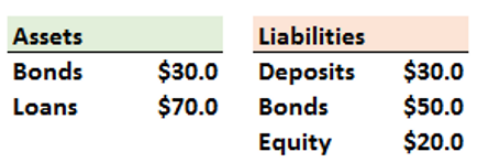
\includegraphics[width=0.4\textwidth]{2·44·1.png.png}
    \end{figure}

    Further, the maturities of these accounts are as follows:
    \begin{itemize}
        \item \textbf{Assets:} The bonds (\$30.0 million) expire in one year. In regard to the loans (\$70.0), \$40.0 million expire in five (5) years, \$10.0 million expire in seven (7) years, and \$20.0 million expire in ten (10) years.
        \item \textbf{Liabilities:} In regard to the deposits (\$30.0 million), \$10.0 million expire in one (1) year, and \$20.0 million expire in two (2) years. In regard to the bonds (\$50.0 million), \$10.0 million expire in five (5) years, \$30.0 million expire in seven (7) years, and \$10.0 million expire in beyond ten ($>10$) years.
        \item \textbf{Equity} (\$20.0 million) is presumed to expire in ten (10) years
    \end{itemize}
    Consider the following possible term structures of expected cash flows:
    \begin{figure}[H]
        \centering
        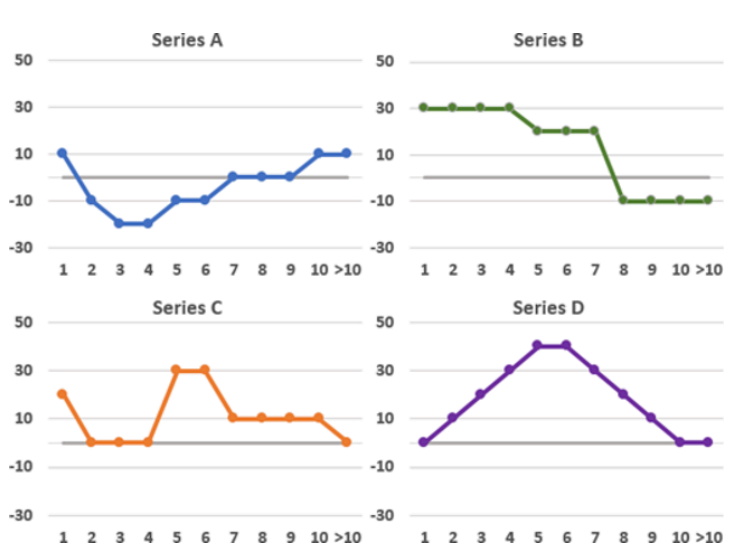
\includegraphics[width=0.4\textwidth]{2·44·2.png.png}
    \end{figure}
    Which term structure of expected cash flows is accurate for Geofinancial Bank?
\end{question}

\begin{choices}
    \item [Option A]
    \item [Option B]
    \item [Option C]
    \item [Option D]
\end{choices}

\begin{correctanswer}
A
\end{correctanswer}

\begin{explanation}
    \textbf{A选项正确。} True: Series A. See below.
    \begin{figure}[H]
        \centering
        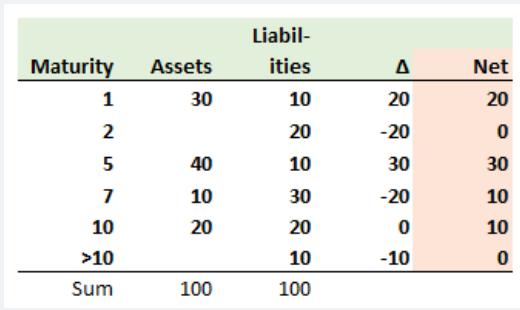
\includegraphics[width=0.6\textwidth]{2·44·3.png}
    \end{figure}
\end{explanation}

\checklist{Finance: Asset Liability Management}{3}{2}


% --- Question 45 ---
\begin{question}
    Acme Industrial Corporation just finished establishing its new financial accounting controls which includes three components: planning, budgeting, and variance monitoring. The company’s next step is to establish a three-legged risk management stool that will analogously include the risk plan, the risk budget, and the risk monitoring process. In regard to the risk plan, each of the following will be an element EXCEPT which is the LEAST likely to be included in Acme’s risk plan?
\end{question}

\begin{choices}
    \item Diversification or risk decomposition policy
    \item Strategic responses for events that are low-probability but franchise-threatening
    \item Ample budget for losses that are material, predictable, and avoidable that cascade down
    \item Identification of critical dependencies that exist inside and outside the organization
\end{choices}

\begin{correctanswer}
    C
\end{correctanswer}

\begin{explanation}
    \textbf{C选项正确。} FALSE. The risk plan should have zero tolerance for mistakes/losses that are “material, predictable, and avoidable.”
    
    In regard to (A), (B), and (D) each is TRUE. According to the authors, the five guideposts in the risk plan are:
    \begin{itemize}
        \item Expected return and volatility goals; and mile posts to recognize failure.
        \item Definition of success or failure
        \item Vision for how risk capital will be deployed; and a diversification or risk decomposition policy
        \item Bright line definition between “merely disappointing events” and seriously damaging losses. Further, “Strategic responses should exist for any franchise-threatening event—even if such events are low-probability situations. The risk plan should identify those types of losses that are so severe that insurance coverage (e.g., asset class puts) should be sought to cover the downside.” (source: 2020 Financial Risk Management Part II: Risk Management and Investment Management, 10th Edition. Pearson Learning Solutions, 2019. VitalBook file.)
        \item Identification of critical dependencies inside and external to the organization
    \end{itemize}
\end{explanation}

\checklist{Financial Risk Management}{3}{2}

% --- Question 46 ---
\begin{question}
    Bertha has a view about correlation, and she is evaluating several rainbow (aka, multi-asset) options. Her view is that correlation is going to decrease. Among the following trades, which \textbf{best} expresses her view?
\end{question}

\begin{choices}
    \item Buy (aka, long position in) basket option
    \item Buy (aka, long position in) better-of-two where payoff = $\max(S_1, S_2)$
    \item Buy correlation (aka, pay the fixed rate) in a correlation swap
    \item Short position in an exchange option where payoff = $\max(0, S_2 - S_1)$
\end{choices}

\begin{correctanswer}
    B
\end{correctanswer}

\begin{explanation}
    \textbf{B选项正确。} Bertha wants to be “short correlation,” and the better-of-two options become more valuable as the correlation decreases. On the other hand:
    \begin{itemize}
        \item The basket option’s value becomes less valuable as the correlation decreases, such that buying the basket option is to be long correlation
        \item Buying correlation (aka, paying the fixed rate) in a correlation swap is long correlation
        \item An exchange option becomes more valuable as the correlation decreases such that a long position in an exchange option is short correlation, and short position in an exchange option is long correlation
    \end{itemize}
\end{explanation}

\checklist{Market Risk: Correlation}{3}{2}

% --- Question 47 ---
\begin{question}
    Julia the analyst is analyzing the credit risk of a contract to which her firm is considering entering into as a party. If true, which feature of her work (among the choices below) \textbf{most likely} signifies or indicates that this is a case of counterparty credit risk rather than (traditional) lending risk or some other type of risk?
\end{question}

\begin{choices}
    \item Interest rate (as a market variable) fluctuations have little impact on the amount owed
    \item The exposure at default (EAD) is 100\% of the notional over most of the life of the contract
    \item Her firm is the only party assuming credit risk: if her firm defaults, the other party faces no losses
    \item She is employing Monte Carlo simulation because the future value of the contract is highly uncertain
\end{choices}

\begin{correctanswer}
D
\end{correctanswer}

\begin{explanation}
    \textbf{D选项正确。} She is employing Monte Carlo simulation because the future value of the contract is highly uncertain.
    
    According to Jon Gregory, the two key differences between counterparty and lending risk are (1) the lender knows the amount at risk but in the case of counterparty risk the amount is highly uncertain, and (2) lending involves unilateral risk (by the lender) but counterparty risk is bilateral to both counterparties.
    
    In regard to false (a), Herstatt risk is a special case (cross-currency) of settlement risk as opposed to pre-settlement risk.
\end{explanation}

    \checklist{Counterparty Credit Risk}{3}{2}

% --- Question 48 ---
\begin{question}
    The Basel regulatory framework has undergone several major renovations but started in the late 1980s when the Basel Committee on Banking Supervision published the first Basel accord, which is now called Basel I; this original Basel I was implemented in 1992. According to Carey (GARP Chapter 19), which BEST summarizes the motivation(s) of the original Basel?
\end{question}

\begin{choices}
    \item To formalize regulatory capital requirements with a set of regulations (i.e., Basel) that would become legal requirements and therefore carried the force of law; i.e., the motivation was legal
    \item Regulators realized that specific measures of short- and long-term liquidity were necessary given that liquidity crunches had been the essential common denominator of recent financial disasters; i.e., the motivation was liquidity
    \item The growth of cross-border finance required both the solvency of banks during stressful periods and fair competition (aka, level playing field) between banks competing in each other's home countries; i.e., the motivations were bank safety and competitive concerns
    \item In the wake of a global recession, there was a motivation to incentivize banks to increase their lending (which had been historically low) in order to grow the developed and emerging economies; i.e., the motivation was economic recovery especially of emerging economies
\end{choices}

\begin{correctanswer}
    C
\end{correctanswer}

\begin{explanation}
    \textbf{Option C is correct.} True: The growth of cross-border finance required both the solvency of banks during stressful periods and fair competition (aka, level playing field) between banks competing in each other's home countries; i.e., the motivations were bank safety and competitive concerns.
    
    Carey explains, ``Two events motivated creation of Basel I.
    \begin{itemize}
        \item First, the growth of cross-border finance continued after Herstatt's failure and it was evident that the G10 nations had a common interest in ensuring that banks had enough equity to absorb large losses.
        \item Second, international banks were competing vigorously in each other's home countries. However, minimum levels of required capital varied significantly across nations, creating a perception that banks headquartered in countries with low minimums had a competitive advantage. In response, members of the BCBS decided to develop a global minimum standard to ``level the playing field'' and avoid a race to the bottom. That is, while the Basel Accord was partly about ensuring safety and soundness, negotiations also had an element of maneuvering for perceived competitive advantage.''
    \end{itemize}
    \textit{(Source: Chapter 19, 2020 FRM Part II: Operational Risk and Resiliency, 10th Edition. Pearson Learning Solutions.)}
\end{explanation}

\checklist{Finance: Basel Accords}{3}{2}

% --- Question 49 ---
\begin{question}
    Which of the following types of liquidity is available in the form of the institution’s liquidity asset buffer (LAB) and represents liquidity available to meet general financial obligations under a stress scenario?
\end{question}

\begin{choices}
    \item Operational
    \item Strategic
    \item Contingent
    \item Restricted
\end{choices}

\begin{correctanswer}
    C
\end{correctanswer}

\begin{explanation}
    \textbf{C选项正确。} Contingent liquidity captures cash or assets that are available when a stressing scenario materializes. The liquidity is contingent on the occurrence of the stress situation. Included within this category are financial assets that can be converted into cash without any material loss in value. Capturing contingent liquidity to cover stressed cash outflows represents the main reason for liquidity stress tests.

    See also the diagram below (inspired by Venkat’s Figure 3.1($\dagger$) but rendered by David Harper in MS Visio).
    \begin{figure}[H]
        \centering
        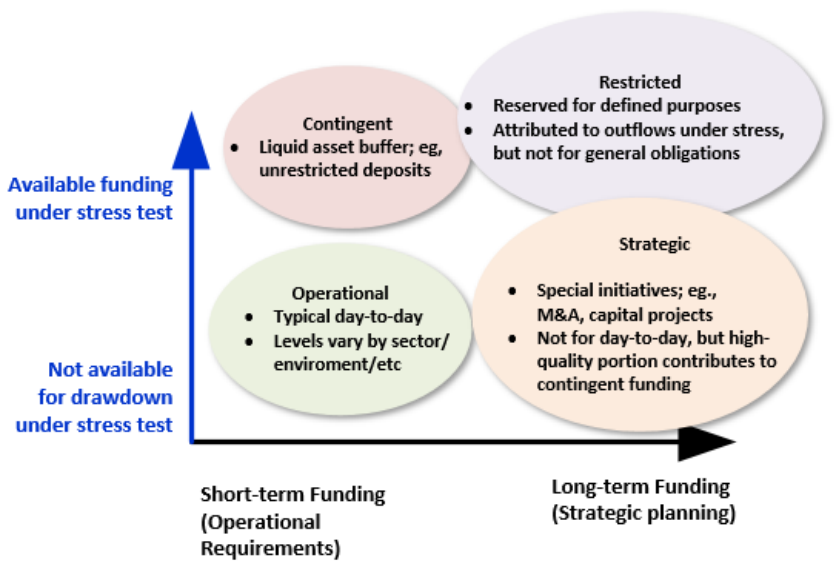
\includegraphics[width=0.6\textwidth]{2·49.png}
    \end{figure}
    Also, writes Venkat (emphasis ours), “\textbf{Liquid asset buffer}: The liquid asset buffer represents the contingent liquidity that is currently in place ... The fundamental characteristics of liquid asset buffer securities should include low credit and market risk, ease and certainty of valuation, trading in an active and sizable market, and low concentration of buyers and sellers. The liquid asset buffer should also meet operational requirements that ensure the liquidity is under the control of the central treasury area of the entity undergoing the stress test.”($\dagger$)
\end{explanation}

\checklist{Finance: Liquidity Risk}{3}{2}

% --- Question 50 ---
\begin{question}
Acme Investment Bank recently finished building the third leg of its three-legged risk management stool, after the risk plan and the risk budget: the bank installed its risk monitoring process. The bank shares a belief with the authors (Rosengarten and Zangari) that “risk is the shadow cost behind returns.” Each of the following is probably an element or plank in the bank’s risk monitoring process EXCEPT which is the least likely to be found in the bank’s risk monitoring process?
\end{question}

\begin{choices}
    \item The bank's monitoring is not dependent on any single tool or metric, but instead relies on an ensemble of various tools and metrics
    \item The bank measures alpha as a regression intercept where alpha can help evaluate manager skill but unfortunately, its statistical significance often requires more data (i.e., longer history) than is available
    \item The bank measures return on risk capital (RORC)) where value at risk (VaR) is a measure of risk capital; in addition to the RORC's level, the bank watches its variability
    \item After a threshold level of data is collected, subjective articulations of each portfolio manager's philosophy becomes unnecessary, and should be discarded, in favor of quantitative performance evaluation
\end{choices}

\begin{correctanswer}
D
\end{correctanswer}

\begin{explanation}
\textbf{Option D is correct.} D. FALSE. Instead, articulation of each portfolio manager's philosophy is always necessary as a complement to quantitative tools and to clarify whether style drift occurs.

As GARP explains in the reading, explicit (and subjective) articulation of philosophy is always a necessary complement to quantitative tools if for no other reason than it helps to identify \textit{style drift}. From the reading: “Before discussing these [i.e., commonly used performance tools], however, it is worth noting that performance tools, while necessary, are not a substitute for timely management intervention when there is an indication of abnormal behavior. By the time that abnormal behavior manifests itself in the form of poor performance statistics, the damage might already be irreversible. For this reason, we believe that performance tools must be supplemented with:
\begin{itemize}
    \item A clear articulation of management philosophy from each portfolio manager. This philosophy statement should identify how the manager expects to extract returns from the market. It should identify ways of knowing when the manager’s process is successful and when it is unsuccessful.
    \item A routine position and style monitoring process designed to identify deviations from philosophy or process. This is a type of early warning system.” — Source: 2020 Financial Risk Management Part II: Risk Management and Investment Management, 10th Edition. Pearson Learning Solutions, 2019. VitalBook file.
\end{itemize}

In regard to (A), (B), and (C), each is TRUE. Specifically,
\begin{itemize}
    \item The bank’s monitoring is not dependent on any single tool or metric, but instead relies on an ensemble of various tools and metrics
    \item The bank measures alpha as a regression intercept where alpha can help evaluate manager skill but unfortunately, its statistical significance often requires more data (i.e., longer history) than is available
    \item The bank measures return on risk capital (RORC)) where value at risk (VaR) is a measure of risk capital; in addition to the RORC’s level, the bank watches its variability
\end{itemize}
\end{explanation}

\checklist{Financial Risk Management}{3}{2}

% --- Question 51 ---
\begin{question}
    Acme FinGlobal Bank has engaged consultants to redefine the organization’s risk measures. The project includes value at risk (VaR) mapping across several portfolios (aka, asset classes) at the organization:
    \begin{itemize}
        \item A fund that invests in initial public offerings (IPOs)
        \item A fund that invests in emergent assets but where with there is little historical data
        \item Small equity portfolio with less than 30 positions
        \item Large equity portfolio with 1,000 positions
        \item A portfolio of corporate bonds that carries six different ratings and has maturities of 3, 5, and 7 years
    \end{itemize}
    Each of the following statements is TRUE except which is false?
\end{question}

\begin{choices}
    \item The corporate bond can be mapped to nine general risk factors
    \item The IPO and emergent asset funds cannot be mapped because these instruments lack historical data such that sensitivities cannot be estimated
    \item The large equity portfolio is an ideal candidate for mapping because mapping to general and specific market primitives requires far fewer numerical estimates than specification of a covariance matrix
    \item The equity portfolio VaR mapping process contains sources of model risk, including factor sensitivities (aka, betas) estimation error, subjective risk factor choices, and specific risk omission
\end{choices}

\begin{correctanswer}
B
\end{correctanswer}

\begin{explanation}
    \textbf{Option B is correct.} False. Instead, mapping is specifically a solution to the problem of insufficient data. As Jorion explains, “The risk manager would have to replace these positions by exposures on similar risk factors already in the system.”$_{(\dagger)}$
    
    In regard to (A), (C), and (D), each is TRUE.
    
    ($\dagger$) Philippe Jorion, Value-at-Risk: The New Benchmark for Managing Financial Risk, 3rd Edition. (New York: McGraw Hill, 2007)
\end{explanation}

\checklist{Market Risk Measurement and Management}{3}{2}

% --- Question 52 ---
\begin{question}
    Freecone Financial LLC entered into an interest rate swap some time ago where it agreed to make semi-annual fixed payments at a rate of $3.0\%$ per annum, in exchange for receiving floating payments on a notional amount of $\$50.0$ million. The floating rate is the six-month secured overnight financing rate (SOFR) and this is also the discount rate used to value the swap. The swap has a remaining life of $1.25$ years. The SOFR rate applicable to the exchange in three months was determined three months ago: it was $2.40\%$. Just as with a LIBOR-based swap, the floating rate is observed at the beginning of each six-month period but paid at the end of the period. Currently, the SOFR term structure is flat at $2.60\%$ per annum with continuous compounding. With respect to its position in this swap, which of the following is nearest to Freecone Financial’s current exposure?
\end{question}

\begin{choices}
    \item Zero
    \item -\$335,900
    \item +\$335,900
    \item +1,335,900
\end{choices}

\begin{correctanswer}
    A
\end{correctanswer}

\begin{explanation}
    \textbf{Option A is correct.} Current exposure = $\max(\text{MtM value}, 0)$. In this case, $\text{CE} = \max(-335,900, 0) = 0$. Freecone is underwater in the swap; its counterparty has positive current exposure because the counterparty experiences a loss in the event of default. But Freecone does not experience a CURRENT loss in the event of default.
\end{explanation}

\checklist{Credit Risk: Current Exposure}{3}{2}

% --- Question 53 ---
\begin{question}
    According to the Guidance on Managing Outsourcing Risk (by the Board of Governors of the Federal Reserve System), with respect to a third-party service provider arrangement, the overall due diligence process by a financial institution should at least include a review of each of the following EXCEPT which is not essential?
\end{question}

\begin{choices}
    \item Ensure service provider has an appropriate background check program for its employees
    \item Financial review of service provider's most recent annual report and financial statements
    \item Evaluate the service provider's performance along environmental, social, and governance (ESG) factors
    \item Evaluate the adequacy of standards, policies and procedures including adherence to applicable laws, regulations and supervisory guidance
\end{choices}

\begin{correctanswer}
    C
\end{correctanswer}

\begin{explanation}
    \textbf{C选项正确。} A review of ESG factors is not mentioned.
    According to the Board, the three broad review areas are:
    \begin{enumerate}
        \item \textit{Business background, reputation, and strategy}: ``Financial institutions should review a prospective service provider's status in the industry and corporate history and qualifications; review the background and reputation of the service provider and its principals; and ensure that the service provider has an appropriate background check program for its employees.''
        \item \textit{Financial performance and condition}: ``Financial institutions should review the financial condition of the service provider and its closely-related affiliates. The financial review may include: The service provider's most recent financial statements and annual report with regard to outstanding commitments, capital strength, liquidity and operating results; The service provider's sustainability, including factors such as the length of time that the service provider has been in business and the service provider's growth of market share for a given service ...''
        \item \textit{Operations and internal controls}.
    \end{enumerate}
\end{explanation}

\checklist{Operational Risk: Outsourcing Risk}{3}{2}

% --- Question 54 ---
\begin{question}
The staff at Umbrella Street Bank, which is a commercial bank (it could also be a savings institution or credit union), produces several liquidity risk reports on a daily, weekly, monthly, and quarterly basis. Among these liquidity risk reports is a deposit tracker report. Among the following metrics, which is MOST LIKELY to appear in their deposit tracker report?
\end{question}

\begin{choices}
    \item Loan-to-deposit (LTD) ratio (current and forecast) versus board-approved lower floor (limit) of $120.0\%$
    \item Loan-to-deposit (LTD) ratio (current and forecast) versus board-approved upper ceiling (limit) of $80.0\%$
    \item Market-to-book ratio of common equity (current and forecast) versus investor-communicated target of $1.30$
    \item The leverage-adjusted duration gap (current and forecast) versus board-approved upper ceiling of $3.5$ years
\end{choices}

\begin{correctanswer}
B
\end{correctanswer}

\begin{explanation}
\textbf{B选项正确。} True: Loan-to-deposit (LTD) ratio (current and forecast) versus board-approved upper ceiling (limit) of $80.0\%$
In regard to (A), (C) and (D), each is FALSE.
\end{explanation}

\checklist{Liquidity Risk Management}{3}{2}

% --- Question 55 ---
\begin{question}
    You work as a pension fund administrator and the Investment Committee asks for your input. The pension fund seeks to increase its allocation to alternative investments and, in particular, will add a new hedge fund strategy; aka, style. You are limited to four strategies. You are perusing the brochures of four hedge funds (each named after Greek gods per a popular marketing convention!). The four strategies are global macro, merger arb, long/short equity, and equity market neutral.

    Below are the four funds. Each fund has a name, a strategy (aka, style), a tagline, and a very brief description.

    \begin{itemize}
        \item \textit{Acheilus} is a Global Macro strategy. We are your effective asset (factor) allocator! We opportunistically make bets in different markets utilizing a range of strategies; you can think of us as betting on a range of factors such as commodities, interest rates, exchange rates.
        \item \textit{Boreas} is a Merger Arb (aka, Risk Arb) strategy. We collect nickels (and dimes) in front of the proverbial steamroller! Like our sibling event-driven strategy (i.e., Distressed), we can offer you nonlinear returns but with tail exposure to extreme market conditions.
        \item \textit{Chimera} is a Long/Short Equity strategy. We are friendly but will never hug a benchmark! Although we have some directional market exposure, we can be classified as relative value because we are stock pickers who seek alpha by way of a diversity of opinions and ability.
        \item \textit{Daphne} is an Equity Market Neutral strategy. We bring you a basket of betas! As an event-driven strategy, our returns are highly linked to several common market risk factors including equity indices, bond spreads, and volatility factors.
    \end{itemize}

    Each of these descriptions is consistent with its strategy (aka, style) category EXCEPT for one. Select the fund that is NOT consistent with its description.
\end{question}

\begin{choices}
    \item Acheilus
    \item Boreas
    \item Chimera
    \item Daphne
\end{choices}

\begin{correctanswer}
    D
\end{correctanswer}

\begin{explanation}
    \textbf{D选项正确。} The tag/description is thrice inconsistent: Equity market neutral is unlinked to observable market risk factors (in the cited research, it is the ONLY strategy found without links to market risk factors). Consequently, an equity market-neutral fund would not ``bring a basket of betas:'' its intention is to neutralize betas; specifically, zero beta with respect to the common market factor. Further, it is not event-driven; equity market-neutral is non-directional and classified as a ``niche strategy'' by the authors, but can also be classified as ``equity hedge.''

    In regard to (A), (B), and (C), each of the other funds (Acheilus, Boreas, and Chimera) have consistent strategies, taglines, and descriptions; i.e., they are conceivably true.
\end{explanation}

\checklist{Finance: Hedge Fund Strategies}{3}{2}

% --- Question 56 ---
\begin{question}
    Betty's firm wants to allocate an economic capital cushion based on a one-day $99.5\%$ value at risk (VaR) model. Further, she will conduct a basic backtest (aka, exception or frequency test) where the frequency of tail losses fit a binomial distribution. Her backtest window is limited to two years, $T = 500$ days. In regard to this backtest, which of the following statements is TRUE?
\end{question}

\begin{choices}
    \item To increase the power of her backtest, she can decrease the VaR confidence level and apply a higher (k) capital multiplier
    \item At this high VaR confidence level and relatively short backtest window, the normal approximation is a better fit to test the model's bias than the binomial distribution
    \item She can achieve a more powerful tests of the same hypothesis, and without the need for any additional information, by utilizing any of several extensions approved by regulators
    \item Although VaR is always a one-tailed quantile (e.g., the $95.0\%$ standard normal VaR is always $1.645$ and never $1.960$), the backtest is always a two-tailed (2T) backtest such that Betty must have a lower and an upper cutoff
\end{choices}

\begin{correctanswer}
    A
\end{correctanswer}

\begin{explanation}
    \textbf{A选项正确。} To increase the power of her backtest, she can decrease the VaR confidence level and apply a higher (k) capital multiplier.
    
    A key statistical challenge for the VaR backtest is that a high confidence level implies a small sample of exceptions. A remedy is to lower the confidence level, but apply a multiplier (to the lower-confidence VaR) in order to approximate a higher-confidence VaR.
    
    As Jorion explains, “The lack of power of this framework is due to the choice of the high VAR confidence level ($99$ percent) that generates too few exceptions for a reliable test. Consider instead the effect of a $95$ percent VAR confidence level. (To ensure that the amount of capital is not affected, we could use a larger multiplier k.)” — Philippe Jorion. Value at Risk, 3rd Ed.: The New Benchmark for Managing Financial Risk (p. 150). Kindle Edition.
    
    In regard to (B), (C) and (D), each is FALSE. Specifically,
    \begin{itemize}
        \item A general guideline for the normal approximation of the binomial is that it can be used when $n \times p$ and $n \times (1-p)$ are greater than $10$; some would say greater than $5$. In this case, $0.5\% \times 500 = 2.5$, such that the binomial probably has too much skew.
        \item The readings (Jorion, Hull or even Dowd) do not reference power gains via regulator-approved extensions
        \item VaR is always a one-tailed quantile (e.g., the $95.0\%$ standard normal VaR is always $1.645$ and never $1.960$), but the backtest is a statistical test and can be either one- or two-tailed (2T)
    \end{itemize}
\end{explanation}

\checklist{Value at Risk (VaR)}{3}{2}

% --- Question 57 ---
\begin{question}
    The figure below illustrates the general role of the credit value adjustment (CVA) desk at Heroic Multifunction Bank (aka, the bank). Assume the trader is a market maker. The uncollateralized trade with the customer (on the left) is hedged with a collateralized trade (on the right):
    \begin{figure}[H]
        \centering
        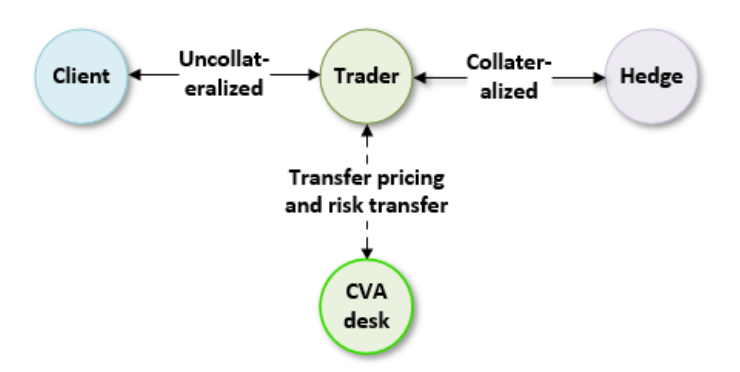
\includegraphics[width=0.6\textwidth]{2·57.png} 
    \end{figure}
    Assume the uncollateralized transaction (with the client) has a positive mark-to-market (MTM) value such that, by definition, the collateralized hedge position, therefore, has a negative MTM value. If the market moves such that, with respect to the position with the client, the position’s positive MTM value INCREASES and becomes even more positive, then which of the following implications is most likely to be TRUE?
\end{question}

\begin{choices}
    \item Funding cost (FVA) is positive
    \item From the trader's (market maker's) perspective, CVA decreases
    \item Because the position is hedged, there is no associated regulatory cost of capital to the bank
    \item The trader (market maker) writes a contingent credit default swap (CCDS) to transfer its counterparty risk
\end{choices}

\begin{correctanswer}
A
\end{correctanswer}

\begin{explanation}
    \textbf{A选项正确。} A. TRUE: Funding cost (FVA) is positive. It will be necessary to post collateral on the hedge and this amount will need to be funded. In regard to (B), (C) and (D), each is FALSE.
    \begin{itemize}
        \item In regard to false (B), CVA is likely to increase as exposure to the further positive position increases
        \item In regard to false (C), their hedge will not eliminate the need for regulatory capital! Says Gregory, “Capital: There will be capital requirements and these will change – which is important because capital is a cost. The capital for the uncollateralised transaction will increase as it becomes in-the-money. The capital for the hedge will not offset this due to being collateralised – and even if it was uncollateralised, there would likely be a convexity impact (the capital for one transaction would increase by more than the capital reduction on the other).”
        \item In regard to false (D), the problem here is that the trader needs to buy (purchase) not write (sell) a CCDS. Says Gregory: “More tailored credit derivative products such as contingent CDS (CCDS) have been designed to hedge counterparty risk even more directly. CCDSs are essentially CDSs but with the notional of protection indexed to the exposure on a contractually specified derivative (or even portfolio of derivatives). They allow the synthetic transfer of counterparty risk linked to a specific trade and counterparty to a third party. However, the CCDS market has never developed any significant liquidity.”
    \end{itemize}
    (Source: Jon Gregory, The xVA Challenge: Counterparty Credit Risk, Funding, Collateral, and Capital, 3rd edition (West Sussex, UK: John Wiley \& Sons, 2015))
\end{explanation}

\checklist{Finance: Counterparty Credit Risk}{3}{2}

% --- Question 58 ---
\begin{question}
    Andrew Ang makes an important, provocative statement when he writes “Reported illiquid asset returns are not returns.” He claims that people overstate the expected returns and understate the risk of illiquid assets, and he attributes this to three key biases. According to Ang, each of the following is a bias that overstates the expected returns (and/or understates the risk) of illiquid assets EXCEPT which is not accurate?
\end{question}

\begin{choices}
    \item Survivorship bias can inflate returns by 4.0\% or more
    \item Infrequent sampling (aka, infrequent trading) artificially reduces risk and risk-related metrics such as volatility, correlation and beta
    \item Turnover bias decreases the typical time between transactions and tends to artificially increase the expected return by 5.0\% or more
    \item Selection bias (aka, reporting bias) is a distortion of the sample that artificially increases (ie, overestimates) alpha and artificially decreases (ie, underestimates) beta
\end{choices}

\begin{correctanswer}
C
\end{correctanswer}

\begin{explanation}
    \textbf{C选项正确。}False. Turnover bias is made-up.
    In regard to (A), (B) and (D), each is TRUE.
    According to Ang , with respect to illiquid assets, the three biases that prompt investor to overstate expect returns while underestimating risk are: survivorship bias; infrequent sampling; and selection bias.
\end{explanation}

\checklist{Alternative Investments: Illiquid Assets}{3}{2}

% --- Question 59 ---
\begin{question}
    Which of the following provides the BEST explicit link(s) between a bank’s contingency funding plan (CFP) and its liquidity stress testing framework?
\end{question}

\begin{choices}
    \item Communication plan
    \item Limit structure and escalation levels
    \item Funding sources concentration and non-core funding
    \item Industry factors such as profitability trends in the financial sector
\end{choices}

\begin{correctanswer}
B
\end{correctanswer}

\begin{explanation}
    \textbf{B选项正确。} True: limit structure and escalation levels
    
    Explain Lai and Tuosto (emphasis ours), “II. Integrate with Broader Risk Management Frameworks: The CFP is not a stand-alone tool, but rather, an integrated part of the institution’s liquidity risk management and firm-wide risk management frameworks ... The CFP should be explicitly linked to the liquidity risk measurement framework and the liquidity stress test, in particular through its limit structure and escalation levels. For example, the liquidity risk measures used in the institution’s BAU risk management activities serve as a foundation from which the CFP defines its early warning indicators (EWIs). Additionally, linkages to the business continuity and crisis management frameworks will reinforce key operational and communication protocols during times of crisis.” — Chi Lai and Richard Tuosto, Contingency Funding Planning in Venkat’s Liquidity Risk Management
\end{explanation}

\checklist{Liquidity Risk Management}{3}{2}

% --- Question 60 ---
\begin{question}
    Bodie, Kane and Marcus explain, based on an analogy originally developed by Robert C. Merton, that we can attempt to quantify the value of market timing by recognizing that foresight is similar to holding a call option on the owned equity portfolio (without paying the premium): the perfect market timer exercises her option, so to speak, by switching from the riskfree asset to the equity portfolio (or vice-versa) depending on which offers the better return. Consequently, the Black-Scholes (BSM) formula can be used, but when the strike price is given by $\$1.00 \cdot \exp(rT)$, the BSM call option formula conveniently reduces to $c = 2 N[0.5 \sigma(e) \sqrt{T}] - 1$.

    If we assume annual forecasts ($T = 1.0$ year), and the volatility of the equity portfolio, $\sigma(e) = 36.0\%$ per annum, which of the following is \textbf{nearest} to the value of perfect market timing, as a percentage of the equity portfolio’s value?
\end{question}

\begin{choices}
    \item 7.39\%
    \item 14.28\%
    \item 46.50\%
    \item 83.77\%
\end{choices}

\begin{correctanswer}
    B
\end{correctanswer}

\begin{explanation}
    \textbf{B选项正确。} In this case, $0.5 \sigma(e) \sqrt{T} = 0.5 \times 36.0\% \times \sqrt{1} = 18.0\% = 0.180$ and $N(0.18) = 0.57140$ if rounded per the lookup table.
    Then $c = 2 \times 0.57140 - 1 = 14.28\%$.
\end{explanation}

\checklist{Portfolio Management}{3}{2}

% --- Question 61 ---
\begin{question}
    Patricia has been asked by the Chief Risk Officer (CRO) to estimate value at risk (VaR) at high confidence levels. Initially, she fits a generalized extreme value (GEV) distribution to the loss data. However, some members of the ultimate audience (the board) do not understand the math. She observes that Dowd($\dagger$) explains, "[t]here are also short-cut ways to estimate VaR (or ES) using EV theory. These are based on the idea that if $\xi > 0$, the tail of an extreme loss distribution follows a power-law times a slowly varying function: $F(x) = k(x)x^{-1/\xi}$ where $k(x)$ varies slowly with $x$. For example, if we assume for convenience that $k(x)$ is approximately constant, then [this equation] becomes: $F(x) \approx k x^{-1/\xi}$". Notice the assumption that $k(x)$ is approximately constant.

    The exponent in Dowd's power law maintains consistency with the generalized extreme value (GEV) distribution by referring to the exponent as a negative reciprocal, $-1/\xi$, but given this exponent is also a constant along with $k(x)$, we can further simplify the approximation: instead of $F(x) \approx k x^{-1/\xi}$, we can say that $F(x) \approx k x^{-\xi}$ which is sometimes represented as $F(x) \approx k x^{-\alpha}$ where $\alpha = 1/\xi$. For example, Patricia assumes the exponent's value is -4.0. In the former syntax, $\xi = 0.25$ such that $(-1/\xi) = -4.0$; in the latter version, $\alpha = 4.0$ such that $(-\alpha) = -4.0$, to the same effect. For our purpose here, we will simply refer to $F(x) \approx k x^{-\xi}$.

    Consequently, she decides to estimate extremely confident VaRs with a power-law shortcut. Specifically, when Patricia sets xi, $\xi = 4.0$, she observes that the 99.50\% VaR is \$6.0 million. With respect to the exponent, she assumes $F(x) \approx k x^{-\xi} = F(x) \approx k x^{-4.0}$. If the loss tail follows the power law, which is \textbf{nearest} to the implied 99.90\% VaR?
\end{question}

\begin{choices}
    \item \$5.0 million
    \item \$9.0 million
    \item \$13.0 million
    \item \$21.0 million
\end{choices}

\begin{correctanswer}
    B
\end{correctanswer}

\begin{explanation}
    \textbf{B选项正确。} We first need to solve for $k$. Dowd($\dagger$) uses an exponent of $(-1/\xi)$ but we shall refer to its simpler reciprocal $(-\xi)$ in the exponent. In this way, the power law says the following: $\text{Prob}(v > x) = F(x) \approx k x^{-\xi}$. Solving for the constant $k$, it must be that: $k = F(x) x^{\xi}$. In this case where we are given that $x = 6.0$ when $F(x) = 0.50\%$ and $\xi = 4.0$, we can find $k = 0.50\% \cdot 6.0^4 = 6.480$. Now we know, because we are assuming constant ($k$) per the approximation, that our distribution is $F(x) \approx k x^{-\xi} = 6.480 x^{-4.0}$. We want the VaR implied by $F(x) = 0.10\%$ such that $0.10\% = 6.480 x^{-4.0}$ where $x = (6.480/0.10\%)^{1/4.0} = 8.97$ which rounds to \$9.0 million.
\end{explanation}

\checklist{Quantitative Analysis: Extreme Value Theory}{3}{2}




















\end{document}